\documentclass[twoside]{book}

% Packages required by doxygen
\usepackage{calc}
\usepackage{doxygen}
\usepackage{graphicx}
\usepackage[utf8]{inputenc}
\usepackage{makeidx}
\usepackage{multicol}
\usepackage{multirow}
\usepackage{textcomp}
\usepackage[table]{xcolor}

% Font selection
\usepackage[T1]{fontenc}
\usepackage{mathptmx}
\usepackage[scaled=.90]{helvet}
\usepackage{courier}
\usepackage{amssymb}
\usepackage{sectsty}
\renewcommand{\familydefault}{\sfdefault}
\allsectionsfont{%
  \fontseries{bc}\selectfont%
  \color{darkgray}%
}
\renewcommand{\DoxyLabelFont}{%
  \fontseries{bc}\selectfont%
  \color{darkgray}%
}

% Page & text layout
\usepackage{geometry}
\geometry{%
  a4paper,%
  top=2.5cm,%
  bottom=2.5cm,%
  left=2.5cm,%
  right=2.5cm%
}
\tolerance=750
\hfuzz=15pt
\hbadness=750
\setlength{\emergencystretch}{15pt}
\setlength{\parindent}{0cm}
\setlength{\parskip}{0.2cm}
\makeatletter
\renewcommand{\paragraph}{%
  \@startsection{paragraph}{4}{0ex}{-1.0ex}{1.0ex}{%
    \normalfont\normalsize\bfseries\SS@parafont%
  }%
}
\renewcommand{\subparagraph}{%
  \@startsection{subparagraph}{5}{0ex}{-1.0ex}{1.0ex}{%
    \normalfont\normalsize\bfseries\SS@subparafont%
  }%
}
\makeatother

% Headers & footers
\usepackage{fancyhdr}
\pagestyle{fancyplain}
\fancyhead[LE]{\fancyplain{}{\bfseries\thepage}}
\fancyhead[CE]{\fancyplain{}{}}
\fancyhead[RE]{\fancyplain{}{\bfseries\leftmark}}
\fancyhead[LO]{\fancyplain{}{\bfseries\rightmark}}
\fancyhead[CO]{\fancyplain{}{}}
\fancyhead[RO]{\fancyplain{}{\bfseries\thepage}}
\fancyfoot[LE]{\fancyplain{}{}}
\fancyfoot[CE]{\fancyplain{}{}}
\fancyfoot[RE]{\fancyplain{}{\bfseries\scriptsize Generated on Fri May 30 2014 15\-:11\-:46 for My Project by Doxygen }}
\fancyfoot[LO]{\fancyplain{}{\bfseries\scriptsize Generated on Fri May 30 2014 15\-:11\-:46 for My Project by Doxygen }}
\fancyfoot[CO]{\fancyplain{}{}}
\fancyfoot[RO]{\fancyplain{}{}}
\renewcommand{\footrulewidth}{0.4pt}
\renewcommand{\chaptermark}[1]{%
  \markboth{#1}{}%
}
\renewcommand{\sectionmark}[1]{%
  \markright{\thesection\ #1}%
}

% Indices & bibliography
\usepackage{natbib}
\usepackage[titles]{tocloft}
\setcounter{tocdepth}{3}
\setcounter{secnumdepth}{5}
\makeindex

% Hyperlinks (required, but should be loaded last)
\usepackage{ifpdf}
\ifpdf
  \usepackage[pdftex,pagebackref=true]{hyperref}
\else
  \usepackage[ps2pdf,pagebackref=true]{hyperref}
\fi
\hypersetup{%
  colorlinks=true,%
  linkcolor=blue,%
  citecolor=blue,%
  unicode%
}

% Custom commands
\newcommand{\clearemptydoublepage}{%
  \newpage{\pagestyle{empty}\cleardoublepage}%
}


%===== C O N T E N T S =====

\begin{document}

% Titlepage & ToC
\hypersetup{pageanchor=false}
\pagenumbering{roman}
\begin{titlepage}
\vspace*{7cm}
\begin{center}%
{\Large My Project }\\
\vspace*{1cm}
{\large Generated by Doxygen 1.8.6}\\
\vspace*{0.5cm}
{\small Fri May 30 2014 15:11:46}\\
\end{center}
\end{titlepage}
\clearemptydoublepage
\tableofcontents
\clearemptydoublepage
\pagenumbering{arabic}
\hypersetup{pageanchor=true}

%--- Begin generated contents ---
\chapter{Class Index}
\section{Class List}
Here are the classes, structs, unions and interfaces with brief descriptions\-:\begin{DoxyCompactList}
\item\contentsline{section}{\hyperlink{classCoinSlot}{Coin\-Slot} }{\pageref{classCoinSlot}}{}
\item\contentsline{section}{\hyperlink{structDestination}{Destination} }{\pageref{structDestination}}{}
\item\contentsline{section}{\hyperlink{classDestinationCollection}{Destination\-Collection} }{\pageref{classDestinationCollection}}{}
\item\contentsline{section}{\hyperlink{classPriceComputer}{Price\-Computer} }{\pageref{classPriceComputer}}{}
\item\contentsline{section}{\hyperlink{classRefoundComputer}{Refound\-Computer} }{\pageref{classRefoundComputer}}{}
\item\contentsline{section}{\hyperlink{classTicketMachine}{Ticket\-Machine} }{\pageref{classTicketMachine}}{}
\end{DoxyCompactList}

\chapter{File Index}
\section{File List}
Here is a list of all files with brief descriptions\-:\begin{DoxyCompactList}
\item\contentsline{section}{\hyperlink{calculator_8cpp}{calculator.\-cpp} }{\pageref{calculator_8cpp}}{}
\item\contentsline{section}{\hyperlink{calculator_8h}{calculator.\-h} }{\pageref{calculator_8h}}{}
\item\contentsline{section}{\hyperlink{console__input_8cpp}{console\-\_\-input.\-cpp} }{\pageref{console__input_8cpp}}{}
\item\contentsline{section}{\hyperlink{console__input_8h}{console\-\_\-input.\-h} }{\pageref{console__input_8h}}{}
\item\contentsline{section}{\hyperlink{fraction_8cpp}{fraction.\-cpp} }{\pageref{fraction_8cpp}}{}
\item\contentsline{section}{\hyperlink{fraction_8h}{fraction.\-h} }{\pageref{fraction_8h}}{}
\item\contentsline{section}{\hyperlink{main_8cpp}{main.\-cpp} }{\pageref{main_8cpp}}{}
\item\contentsline{section}{\hyperlink{main_8h}{main.\-h} }{\pageref{main_8h}}{}
\end{DoxyCompactList}

\chapter{Class Documentation}
\hypertarget{classCoinSlot}{\section{Coin\-Slot Class Reference}
\label{classCoinSlot}\index{Coin\-Slot@{Coin\-Slot}}
}


{\ttfamily \#include $<$coin\-\_\-slot.\-h$>$}

\subsection*{Public Member Functions}
\begin{DoxyCompactItemize}
\item 
\hyperlink{classCoinSlot_a7ee2abc60da5a7af641eff10c5c4c2bf}{Coin\-Slot} ()
\item 
\hyperlink{classCoinSlot_a0b2fe39a7b9e9d13df98735a85af986c}{Coin\-Slot} (const string \&a\-\_\-currency)
\item 
\hyperlink{classCoinSlot_ae3fcb033d930eb7827649e2740275aca}{Coin\-Slot} (const string \&a\-\_\-currency, const vector$<$ double $>$ \&accepted\-\_\-coins\-\_\-list)
\item 
void \hyperlink{classCoinSlot_aeb67f3b2b68ed5c22c1d6f192f315104}{insert} (double a\-\_\-coin)  throw (const invalid\-\_\-argument)
\item 
void \hyperlink{classCoinSlot_a8ed8cda62086c21f647d215f47d31b3b}{add\-\_\-accepted} (double a\-\_\-coin)
\item 
double \hyperlink{classCoinSlot_aa349eea94746d3438335c7ef5337bf7c}{get\-\_\-value} () const 
\item 
string \hyperlink{classCoinSlot_af37381120a0315178139de6ce447741d}{str} () const 
\end{DoxyCompactItemize}


\subsection{Detailed Description}
\hyperlink{classCoinSlot}{Coin\-Slot} represents a coin slot of a ticket machine. You can define certain accepted coins. When inserting a coin (double), it validates for acceptance. The class also overrides the global operators $>$$>$ \char`\"{}get from\char`\"{} and $<$$<$ \char`\"{}put to\char`\"{} for easy console input handling.

\begin{DoxyAuthor}{Author}
Lukas Hodel 
\end{DoxyAuthor}
\begin{DoxyVersion}{Version}
1.\-0 
\end{DoxyVersion}


\subsection{Constructor \& Destructor Documentation}
\hypertarget{classCoinSlot_a7ee2abc60da5a7af641eff10c5c4c2bf}{\index{Coin\-Slot@{Coin\-Slot}!Coin\-Slot@{Coin\-Slot}}
\index{Coin\-Slot@{Coin\-Slot}!CoinSlot@{Coin\-Slot}}
\subsubsection[{Coin\-Slot}]{\setlength{\rightskip}{0pt plus 5cm}Coin\-Slot\-::\-Coin\-Slot (
\begin{DoxyParamCaption}
{}
\end{DoxyParamCaption}
)}}\label{classCoinSlot_a7ee2abc60da5a7af641eff10c5c4c2bf}
Empty constructor, initializes a \hyperlink{classCoinSlot}{Coin\-Slot} with the currency \char`\"{}\-Euro\char`\"{} and accepts no coins. \hypertarget{classCoinSlot_a0b2fe39a7b9e9d13df98735a85af986c}{\index{Coin\-Slot@{Coin\-Slot}!Coin\-Slot@{Coin\-Slot}}
\index{Coin\-Slot@{Coin\-Slot}!CoinSlot@{Coin\-Slot}}
\subsubsection[{Coin\-Slot}]{\setlength{\rightskip}{0pt plus 5cm}Coin\-Slot\-::\-Coin\-Slot (
\begin{DoxyParamCaption}
\item[{const string \&}]{a\-\_\-currency}
\end{DoxyParamCaption}
)}}\label{classCoinSlot_a0b2fe39a7b9e9d13df98735a85af986c}
Constructor, initializes a \hyperlink{classCoinSlot}{Coin\-Slot} with a given currency. It accepts no coins.


\begin{DoxyParams}{Parameters}
{\em a\-\_\-currency} & currency of the coins. \\
\hline
\end{DoxyParams}
\hypertarget{classCoinSlot_ae3fcb033d930eb7827649e2740275aca}{\index{Coin\-Slot@{Coin\-Slot}!Coin\-Slot@{Coin\-Slot}}
\index{Coin\-Slot@{Coin\-Slot}!CoinSlot@{Coin\-Slot}}
\subsubsection[{Coin\-Slot}]{\setlength{\rightskip}{0pt plus 5cm}Coin\-Slot\-::\-Coin\-Slot (
\begin{DoxyParamCaption}
\item[{const string \&}]{a\-\_\-currency, }
\item[{const vector$<$ double $>$ \&}]{accepted\-\_\-coins\-\_\-list}
\end{DoxyParamCaption}
)}}\label{classCoinSlot_ae3fcb033d930eb7827649e2740275aca}
Constructor, inizializes a \hyperlink{classCoinSlot}{Coin\-Slot} with a given currency and a list of accepted coins.


\begin{DoxyParams}{Parameters}
{\em a\-\_\-currency} & Currency of the coins. \\
\hline
{\em accepted\-\_\-coins\-\_\-list} & List of accepted coins. \\
\hline
\end{DoxyParams}


\subsection{Member Function Documentation}
\hypertarget{classCoinSlot_a8ed8cda62086c21f647d215f47d31b3b}{\index{Coin\-Slot@{Coin\-Slot}!add\-\_\-accepted@{add\-\_\-accepted}}
\index{add\-\_\-accepted@{add\-\_\-accepted}!CoinSlot@{Coin\-Slot}}
\subsubsection[{add\-\_\-accepted}]{\setlength{\rightskip}{0pt plus 5cm}void Coin\-Slot\-::add\-\_\-accepted (
\begin{DoxyParamCaption}
\item[{double}]{a\-\_\-coin}
\end{DoxyParamCaption}
)}}\label{classCoinSlot_a8ed8cda62086c21f647d215f47d31b3b}
Adds a coin to the list of accepted coins.


\begin{DoxyParams}{Parameters}
{\em a\-\_\-coin} & Coin which should be accepted by the \hyperlink{classCoinSlot}{Coin\-Slot}. \\
\hline
\end{DoxyParams}
\hypertarget{classCoinSlot_aa349eea94746d3438335c7ef5337bf7c}{\index{Coin\-Slot@{Coin\-Slot}!get\-\_\-value@{get\-\_\-value}}
\index{get\-\_\-value@{get\-\_\-value}!CoinSlot@{Coin\-Slot}}
\subsubsection[{get\-\_\-value}]{\setlength{\rightskip}{0pt plus 5cm}double Coin\-Slot\-::get\-\_\-value (
\begin{DoxyParamCaption}
{}
\end{DoxyParamCaption}
) const}}\label{classCoinSlot_aa349eea94746d3438335c7ef5337bf7c}
Returns the value of the inserted coin.

\begin{DoxyReturn}{Returns}
value of the inserted coin. 
\end{DoxyReturn}
\hypertarget{classCoinSlot_aeb67f3b2b68ed5c22c1d6f192f315104}{\index{Coin\-Slot@{Coin\-Slot}!insert@{insert}}
\index{insert@{insert}!CoinSlot@{Coin\-Slot}}
\subsubsection[{insert}]{\setlength{\rightskip}{0pt plus 5cm}void Coin\-Slot\-::insert (
\begin{DoxyParamCaption}
\item[{double}]{a\-\_\-coin}
\end{DoxyParamCaption}
)  throw (const invalid\-\_\-argument)}}\label{classCoinSlot_aeb67f3b2b68ed5c22c1d6f192f315104}
Insert a coin into the coin slot. Checks if the coin is accepted.


\begin{DoxyParams}{Parameters}
{\em a\-\_\-coin} & Coin to insert into the coin slot.\\
\hline
\end{DoxyParams}

\begin{DoxyExceptions}{Exceptions}
{\em std\-::invalid\-\_\-argument} & when coin is not accepted. \\
\hline
\end{DoxyExceptions}
\hypertarget{classCoinSlot_af37381120a0315178139de6ce447741d}{\index{Coin\-Slot@{Coin\-Slot}!str@{str}}
\index{str@{str}!CoinSlot@{Coin\-Slot}}
\subsubsection[{str}]{\setlength{\rightskip}{0pt plus 5cm}string Coin\-Slot\-::str (
\begin{DoxyParamCaption}
{}
\end{DoxyParamCaption}
) const}}\label{classCoinSlot_af37381120a0315178139de6ce447741d}
Represents the \hyperlink{classCoinSlot}{Coin\-Slot} as a string. It shows a list of the accepted coins.

Moegliche Zahlungseinehten\-: 50.\-00 Euro 20.\-00 Euro ...

\begin{DoxyReturn}{Returns}
String with the list of the accepted coins. 
\end{DoxyReturn}


The documentation for this class was generated from the following files\-:\begin{DoxyCompactItemize}
\item 
\hyperlink{coin__slot_8h}{coin\-\_\-slot.\-h}\item 
\hyperlink{coin__slot_8cpp}{coin\-\_\-slot.\-cpp}\end{DoxyCompactItemize}

\hypertarget{structDestination}{\section{Destination Struct Reference}
\label{structDestination}\index{Destination@{Destination}}
}


{\ttfamily \#include $<$destination.\-h$>$}

\subsection*{Public Attributes}
\begin{DoxyCompactItemize}
\item 
string \hyperlink{structDestination_a06f463b8bcd6e5ae0c73e36e8f888f1f}{name}
\item 
float \hyperlink{structDestination_ae1f8135f13ad4a30f519ef4c85cf4a1a}{price}
\item 
string \hyperlink{structDestination_af1050e1a2a7f928ffc9a18ee8942292d}{currency}
\end{DoxyCompactItemize}


\subsection{Detailed Description}
Represents a destination for a ticket machine. 

\subsection{Member Data Documentation}
\hypertarget{structDestination_af1050e1a2a7f928ffc9a18ee8942292d}{\index{Destination@{Destination}!currency@{currency}}
\index{currency@{currency}!Destination@{Destination}}
\subsubsection[{currency}]{\setlength{\rightskip}{0pt plus 5cm}string Destination\-::currency}}\label{structDestination_af1050e1a2a7f928ffc9a18ee8942292d}
\hypertarget{structDestination_a06f463b8bcd6e5ae0c73e36e8f888f1f}{\index{Destination@{Destination}!name@{name}}
\index{name@{name}!Destination@{Destination}}
\subsubsection[{name}]{\setlength{\rightskip}{0pt plus 5cm}string Destination\-::name}}\label{structDestination_a06f463b8bcd6e5ae0c73e36e8f888f1f}
\hypertarget{structDestination_ae1f8135f13ad4a30f519ef4c85cf4a1a}{\index{Destination@{Destination}!price@{price}}
\index{price@{price}!Destination@{Destination}}
\subsubsection[{price}]{\setlength{\rightskip}{0pt plus 5cm}float Destination\-::price}}\label{structDestination_ae1f8135f13ad4a30f519ef4c85cf4a1a}


The documentation for this struct was generated from the following file\-:\begin{DoxyCompactItemize}
\item 
\hyperlink{destination_8h}{destination.\-h}\end{DoxyCompactItemize}

\hypertarget{classDestinationCollection}{\section{Destination\-Collection Class Reference}
\label{classDestinationCollection}\index{Destination\-Collection@{Destination\-Collection}}
}


{\ttfamily \#include $<$destination\-\_\-collection.\-h$>$}

\subsection*{Public Member Functions}
\begin{DoxyCompactItemize}
\item 
\hyperlink{classDestinationCollection_a8cd302a3be128dde1c742a40268d0768}{Destination\-Collection} ()
\item 
\hyperlink{classDestinationCollection_ab31794d8d9769b43d4c903f4e835b8be}{Destination\-Collection} (string a\-\_\-currency)
\item 
int \hyperlink{classDestinationCollection_abe6e5181031cc5db9bac4b6a39000964}{add} (string name, float price)
\item 
void \hyperlink{classDestinationCollection_a764aaa3f333fc5d0bc6101e35e2bfbaa}{remove} (int key)
\item 
void \hyperlink{classDestinationCollection_a27de949dd04a84f108f246a579b22fdc}{clear} ()
\item 
int \hyperlink{classDestinationCollection_a35325e80b3ba8d6e935c7474463c9434}{size} () const 
\item 
\hyperlink{structDestination}{Destination} \hyperlink{classDestinationCollection_af0552ec87e81f036994e8d9838bc36ea}{operator\mbox{[}$\,$\mbox{]}} (int key) const 
\end{DoxyCompactItemize}


\subsection{Detailed Description}
\hyperlink{classDestinationCollection}{Destination\-Collection} represents a collection of Destinations. Destinations is a struct with the data fields name and price.

\begin{DoxyAuthor}{Author}
Lukas Hodel 
\end{DoxyAuthor}
\begin{DoxyVersion}{Version}
1.\-0 
\end{DoxyVersion}


\subsection{Constructor \& Destructor Documentation}
\hypertarget{classDestinationCollection_a8cd302a3be128dde1c742a40268d0768}{\index{Destination\-Collection@{Destination\-Collection}!Destination\-Collection@{Destination\-Collection}}
\index{Destination\-Collection@{Destination\-Collection}!DestinationCollection@{Destination\-Collection}}
\subsubsection[{Destination\-Collection}]{\setlength{\rightskip}{0pt plus 5cm}Destination\-Collection\-::\-Destination\-Collection (
\begin{DoxyParamCaption}
{}
\end{DoxyParamCaption}
)}}\label{classDestinationCollection_a8cd302a3be128dde1c742a40268d0768}
Constructor without parameters initializes a empty collection with the currency as \char`\"{}\-Euro\char`\"{}. \hypertarget{classDestinationCollection_ab31794d8d9769b43d4c903f4e835b8be}{\index{Destination\-Collection@{Destination\-Collection}!Destination\-Collection@{Destination\-Collection}}
\index{Destination\-Collection@{Destination\-Collection}!DestinationCollection@{Destination\-Collection}}
\subsubsection[{Destination\-Collection}]{\setlength{\rightskip}{0pt plus 5cm}Destination\-Collection\-::\-Destination\-Collection (
\begin{DoxyParamCaption}
\item[{string}]{a\-\_\-currency}
\end{DoxyParamCaption}
)}}\label{classDestinationCollection_ab31794d8d9769b43d4c903f4e835b8be}
Constructor without parameters initializes a empty collection with a given currency. 

\subsection{Member Function Documentation}
\hypertarget{classDestinationCollection_abe6e5181031cc5db9bac4b6a39000964}{\index{Destination\-Collection@{Destination\-Collection}!add@{add}}
\index{add@{add}!DestinationCollection@{Destination\-Collection}}
\subsubsection[{add}]{\setlength{\rightskip}{0pt plus 5cm}int Destination\-Collection\-::add (
\begin{DoxyParamCaption}
\item[{string}]{name, }
\item[{float}]{price}
\end{DoxyParamCaption}
)}}\label{classDestinationCollection_abe6e5181031cc5db9bac4b6a39000964}
Adds a new destination to the collection.


\begin{DoxyParams}{Parameters}
{\em name} & Name of the destination. \\
\hline
{\em price} & Fare price to the destination.\\
\hline
\end{DoxyParams}
\begin{DoxyReturn}{Returns}
the new size of the collection counted from zero. 
\end{DoxyReturn}
\hypertarget{classDestinationCollection_a27de949dd04a84f108f246a579b22fdc}{\index{Destination\-Collection@{Destination\-Collection}!clear@{clear}}
\index{clear@{clear}!DestinationCollection@{Destination\-Collection}}
\subsubsection[{clear}]{\setlength{\rightskip}{0pt plus 5cm}void Destination\-Collection\-::clear (
\begin{DoxyParamCaption}
{}
\end{DoxyParamCaption}
)}}\label{classDestinationCollection_a27de949dd04a84f108f246a579b22fdc}
Removes all the destinations from the collection. \hypertarget{classDestinationCollection_af0552ec87e81f036994e8d9838bc36ea}{\index{Destination\-Collection@{Destination\-Collection}!operator\mbox{[}$\,$\mbox{]}@{operator[]}}
\index{operator\mbox{[}$\,$\mbox{]}@{operator[]}!DestinationCollection@{Destination\-Collection}}
\subsubsection[{operator[]}]{\setlength{\rightskip}{0pt plus 5cm}{\bf Destination} Destination\-Collection\-::operator\mbox{[}$\,$\mbox{]} (
\begin{DoxyParamCaption}
\item[{int}]{key}
\end{DoxyParamCaption}
) const}}\label{classDestinationCollection_af0552ec87e81f036994e8d9838bc36ea}
Overrides operator\mbox{[}\mbox{]}. Gives back the destination of the collection at the index of the given key.


\begin{DoxyParams}{Parameters}
{\em key} & Index of the destination to return.\\
\hline
\end{DoxyParams}
\begin{DoxyReturn}{Returns}
\hyperlink{structDestination}{Destination} at the index of the given key. 
\end{DoxyReturn}
\hypertarget{classDestinationCollection_a764aaa3f333fc5d0bc6101e35e2bfbaa}{\index{Destination\-Collection@{Destination\-Collection}!remove@{remove}}
\index{remove@{remove}!DestinationCollection@{Destination\-Collection}}
\subsubsection[{remove}]{\setlength{\rightskip}{0pt plus 5cm}void Destination\-Collection\-::remove (
\begin{DoxyParamCaption}
\item[{int}]{key}
\end{DoxyParamCaption}
)}}\label{classDestinationCollection_a764aaa3f333fc5d0bc6101e35e2bfbaa}
\hypertarget{classDestinationCollection_a35325e80b3ba8d6e935c7474463c9434}{\index{Destination\-Collection@{Destination\-Collection}!size@{size}}
\index{size@{size}!DestinationCollection@{Destination\-Collection}}
\subsubsection[{size}]{\setlength{\rightskip}{0pt plus 5cm}int Destination\-Collection\-::size (
\begin{DoxyParamCaption}
{}
\end{DoxyParamCaption}
) const}}\label{classDestinationCollection_a35325e80b3ba8d6e935c7474463c9434}
Returns the size of the collection with the count start of 1.

\begin{DoxyReturn}{Returns}
size of the collection. 
\end{DoxyReturn}


The documentation for this class was generated from the following files\-:\begin{DoxyCompactItemize}
\item 
\hyperlink{destination__collection_8h}{destination\-\_\-collection.\-h}\item 
\hyperlink{destination__collection_8cpp}{destination\-\_\-collection.\-cpp}\end{DoxyCompactItemize}

\hypertarget{classPriceComputer}{\section{Price\-Computer Class Reference}
\label{classPriceComputer}\index{Price\-Computer@{Price\-Computer}}
}


{\ttfamily \#include $<$price\-\_\-computer.\-h$>$}

\subsection*{Public Member Functions}
\begin{DoxyCompactItemize}
\item 
\hyperlink{classPriceComputer_ad20398c1f27e2ee28bf698ee968417ef}{Price\-Computer} (double a\-\_\-price, string a\-\_\-currency)  throw (const invalid\-\_\-argument)
\item 
double \hyperlink{classPriceComputer_a5432eb25a9dc564e26d28f8c992edc54}{add} (double a\-\_\-coin)  throw (const invalid\-\_\-argument)
\item 
int \hyperlink{classPriceComputer_acd1ed2559f6c99b66877dc176a7f067b}{state} () const 
\item 
double \hyperlink{classPriceComputer_aaafb5acfbdb3419e873d30ff7c544a9e}{remainder} () const 
\item 
string \hyperlink{classPriceComputer_ac6a85d7316a174de19a4eccdffd91ae3}{str} () const 
\end{DoxyCompactItemize}


\subsection{Detailed Description}
\hyperlink{classPriceComputer}{Price\-Computer} is a state machine for counting monetary units up to a certain value.

\begin{DoxyAuthor}{Author}
Lukas Hodel 
\end{DoxyAuthor}


\subsection{Constructor \& Destructor Documentation}
\hypertarget{classPriceComputer_ad20398c1f27e2ee28bf698ee968417ef}{\index{Price\-Computer@{Price\-Computer}!Price\-Computer@{Price\-Computer}}
\index{Price\-Computer@{Price\-Computer}!PriceComputer@{Price\-Computer}}
\subsubsection[{Price\-Computer}]{\setlength{\rightskip}{0pt plus 5cm}Price\-Computer\-::\-Price\-Computer (
\begin{DoxyParamCaption}
\item[{double}]{a\-\_\-price, }
\item[{string}]{a\-\_\-currency}
\end{DoxyParamCaption}
) throw  const invalid\-\_\-argument) }}\label{classPriceComputer_ad20398c1f27e2ee28bf698ee968417ef}
Constructor to initialize a \hyperlink{classPriceComputer}{Price\-Computer} with a given prive and a given currency.


\begin{DoxyParams}{Parameters}
{\em a\-\_\-price} & Price to count to. \\
\hline
{\em a\-\_\-currency} & Currency of the price. \\
\hline
\end{DoxyParams}


\subsection{Member Function Documentation}
\hypertarget{classPriceComputer_a5432eb25a9dc564e26d28f8c992edc54}{\index{Price\-Computer@{Price\-Computer}!add@{add}}
\index{add@{add}!PriceComputer@{Price\-Computer}}
\subsubsection[{add}]{\setlength{\rightskip}{0pt plus 5cm}double Price\-Computer\-::add (
\begin{DoxyParamCaption}
\item[{double}]{a\-\_\-coin}
\end{DoxyParamCaption}
) throw  const invalid\-\_\-argument) }}\label{classPriceComputer_a5432eb25a9dc564e26d28f8c992edc54}
Adds a coin \char`\"{}value\char`\"{} to the \hyperlink{classPriceComputer}{Price\-Computer}. Gets summed by previous added coins.


\begin{DoxyParams}{Parameters}
{\em a\-\_\-coin} & Coin \char`\"{}value\char`\"{} to add.\\
\hline
\end{DoxyParams}
\begin{DoxyReturn}{Returns}
sum of all added coins until now. 
\end{DoxyReturn}
\hypertarget{classPriceComputer_aaafb5acfbdb3419e873d30ff7c544a9e}{\index{Price\-Computer@{Price\-Computer}!remainder@{remainder}}
\index{remainder@{remainder}!PriceComputer@{Price\-Computer}}
\subsubsection[{remainder}]{\setlength{\rightskip}{0pt plus 5cm}double Price\-Computer\-::remainder (
\begin{DoxyParamCaption}
{}
\end{DoxyParamCaption}
) const}}\label{classPriceComputer_aaafb5acfbdb3419e873d30ff7c544a9e}
Returns the remainder from the sum of all added coins to the price. Can be negative, when the sum of all coins is higher then the price.

\begin{DoxyReturn}{Returns}
remainder from the sum of all added coins to the price. 
\end{DoxyReturn}
\hypertarget{classPriceComputer_acd1ed2559f6c99b66877dc176a7f067b}{\index{Price\-Computer@{Price\-Computer}!state@{state}}
\index{state@{state}!PriceComputer@{Price\-Computer}}
\subsubsection[{state}]{\setlength{\rightskip}{0pt plus 5cm}int Price\-Computer\-::state (
\begin{DoxyParamCaption}
{}
\end{DoxyParamCaption}
) const}}\label{classPriceComputer_acd1ed2559f6c99b66877dc176a7f067b}
Returns the state of the \hyperlink{classPriceComputer}{Price\-Computer}. There are four different states represented as integers (-\/1, 0, 1 and 2).

\begin{DoxyReturn}{Returns}
state as Integer -\/1 The sum of all added coins is less than the price. 0 Abordet, as soon as a 0.\-00 value coin gets added. 1 The sum of all added coins is exactly the price. 2 The sum of all added coins is more than the price. 
\end{DoxyReturn}
\hypertarget{classPriceComputer_ac6a85d7316a174de19a4eccdffd91ae3}{\index{Price\-Computer@{Price\-Computer}!str@{str}}
\index{str@{str}!PriceComputer@{Price\-Computer}}
\subsubsection[{str}]{\setlength{\rightskip}{0pt plus 5cm}string Price\-Computer\-::str (
\begin{DoxyParamCaption}
{}
\end{DoxyParamCaption}
) const}}\label{classPriceComputer_ac6a85d7316a174de19a4eccdffd91ae3}
Representation of a \hyperlink{classPriceComputer}{Price\-Computer} object as a string. Has a differen output for every state.

when state is -\/1\-: Noch zu bezahlen\-: remainder currency when state is 0\-: Rückgabe\-: sum of all entered coins Zalungseinheiten\-: 1 $\ast$ 50.\-00 Euro 2 $\ast$ 5.\-00 Euro ... When state is 1\-: Nothing When state is 2\-: Zu viel bezahlt! 3.\-30 Euro

\begin{DoxyReturn}{Returns}
Stringrepresentation according the different states. 
\end{DoxyReturn}


Here is the call graph for this function\-:\nopagebreak
\begin{figure}[H]
\begin{center}
\leavevmode
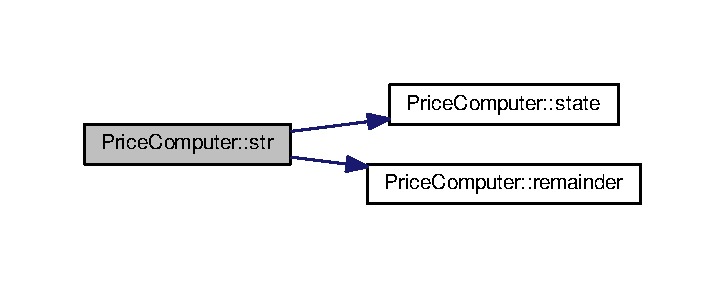
\includegraphics[width=348pt]{classPriceComputer_ac6a85d7316a174de19a4eccdffd91ae3_cgraph}
\end{center}
\end{figure}




The documentation for this class was generated from the following files\-:\begin{DoxyCompactItemize}
\item 
\hyperlink{price__computer_8h}{price\-\_\-computer.\-h}\item 
\hyperlink{price__computer_8cpp}{price\-\_\-computer.\-cpp}\end{DoxyCompactItemize}

\hypertarget{classRefoundComputer}{\section{Refound\-Computer Class Reference}
\label{classRefoundComputer}\index{Refound\-Computer@{Refound\-Computer}}
}


{\ttfamily \#include $<$refound\-\_\-computer.\-h$>$}

\subsection*{Public Member Functions}
\begin{DoxyCompactItemize}
\item 
\hyperlink{classRefoundComputer_a48f52d711a12490074da778084fa9b19}{Refound\-Computer} ()
\item 
\hyperlink{classRefoundComputer_aacf86566e78253410eb02e577664789f}{Refound\-Computer} (const string \&currency, const vector$<$ double $>$ \&accepted\-\_\-coins\-\_\-list)
\item 
void \hyperlink{classRefoundComputer_a2ed7a4501d14097325c5575fa3c5eab7}{set\-\_\-refound} (double a\-\_\-refound)
\item 
string \hyperlink{classRefoundComputer_a94f386e9c403ffc5e47e50628be4731f}{str} () const 
\end{DoxyCompactItemize}


\subsection{Detailed Description}
\hyperlink{classRefoundComputer}{Refound\-Computer} represents the sum of a refound with a list of accepted values.

\begin{DoxyAuthor}{Author}
Lukas Hodel 
\end{DoxyAuthor}
\begin{DoxyVersion}{Version}
1.\-0 
\end{DoxyVersion}


\subsection{Constructor \& Destructor Documentation}
\hypertarget{classRefoundComputer_a48f52d711a12490074da778084fa9b19}{\index{Refound\-Computer@{Refound\-Computer}!Refound\-Computer@{Refound\-Computer}}
\index{Refound\-Computer@{Refound\-Computer}!RefoundComputer@{Refound\-Computer}}
\subsubsection[{Refound\-Computer}]{\setlength{\rightskip}{0pt plus 5cm}Refound\-Computer\-::\-Refound\-Computer (
\begin{DoxyParamCaption}
{}
\end{DoxyParamCaption}
)}}\label{classRefoundComputer_a48f52d711a12490074da778084fa9b19}
Initializes a \hyperlink{classRefoundComputer}{Refound\-Computer} instance with a refound of zero, the currency \char`\"{}\-Euro\char`\"{} and a empty list of accepted values. \hypertarget{classRefoundComputer_aacf86566e78253410eb02e577664789f}{\index{Refound\-Computer@{Refound\-Computer}!Refound\-Computer@{Refound\-Computer}}
\index{Refound\-Computer@{Refound\-Computer}!RefoundComputer@{Refound\-Computer}}
\subsubsection[{Refound\-Computer}]{\setlength{\rightskip}{0pt plus 5cm}Refound\-Computer\-::\-Refound\-Computer (
\begin{DoxyParamCaption}
\item[{const string \&}]{a\-\_\-currency, }
\item[{const vector$<$ double $>$ \&}]{accepted\-\_\-coins\-\_\-list}
\end{DoxyParamCaption}
)}}\label{classRefoundComputer_aacf86566e78253410eb02e577664789f}
Initializes a Refound\-Coumputer instance with a given currency and a given list of accepted values.


\begin{DoxyParams}{Parameters}
{\em a\-\_\-currency} & the currency for string representation. \\
\hline
{\em accepted\-\_\-coins\-\_\-list} & list of accepted values to represent the refound. \\
\hline
\end{DoxyParams}


\subsection{Member Function Documentation}
\hypertarget{classRefoundComputer_a2ed7a4501d14097325c5575fa3c5eab7}{\index{Refound\-Computer@{Refound\-Computer}!set\-\_\-refound@{set\-\_\-refound}}
\index{set\-\_\-refound@{set\-\_\-refound}!RefoundComputer@{Refound\-Computer}}
\subsubsection[{set\-\_\-refound}]{\setlength{\rightskip}{0pt plus 5cm}void Refound\-Computer\-::set\-\_\-refound (
\begin{DoxyParamCaption}
\item[{double}]{a\-\_\-refound}
\end{DoxyParamCaption}
)}}\label{classRefoundComputer_a2ed7a4501d14097325c5575fa3c5eab7}
Sets the refound to represent through the accepted values. and calculates the the sum out of the accepted values.


\begin{DoxyParams}{Parameters}
{\em a\-\_\-refound} & Refound to calculate. \\
\hline
\end{DoxyParams}
\hypertarget{classRefoundComputer_a94f386e9c403ffc5e47e50628be4731f}{\index{Refound\-Computer@{Refound\-Computer}!str@{str}}
\index{str@{str}!RefoundComputer@{Refound\-Computer}}
\subsubsection[{str}]{\setlength{\rightskip}{0pt plus 5cm}string Refound\-Computer\-::str (
\begin{DoxyParamCaption}
{}
\end{DoxyParamCaption}
) const}}\label{classRefoundComputer_a94f386e9c403ffc5e47e50628be4731f}
Returns the representation of the \hyperlink{classRefoundComputer}{Refound\-Computer} as a string. When there are no values calculated for the refound, there will be a empty string. When there is a combination of values calculated, it will return a string like this\-:

Rückgabe\-: 10.\-10 Zahlungseinheigen\-: 1 $\ast$ 10 Euro 1 $\ast$ 0.\-00 Euro.

\begin{DoxyReturn}{Returns}
string representation of the \hyperlink{classRefoundComputer}{Refound\-Computer}. 
\end{DoxyReturn}


The documentation for this class was generated from the following files\-:\begin{DoxyCompactItemize}
\item 
\hyperlink{refound__computer_8h}{refound\-\_\-computer.\-h}\item 
\hyperlink{refound__computer_8cpp}{refound\-\_\-computer.\-cpp}\end{DoxyCompactItemize}

\hypertarget{classTicketMachine}{\section{Ticket\-Machine Class Reference}
\label{classTicketMachine}\index{Ticket\-Machine@{Ticket\-Machine}}
}


{\ttfamily \#include $<$ticket\-\_\-machine.\-h$>$}

\subsection*{Public Member Functions}
\begin{DoxyCompactItemize}
\item 
\hyperlink{classTicketMachine_ad69449ce9b776af44f68482916351186}{Ticket\-Machine} (const string \&a\-\_\-name, const string \&a\-\_\-currency, const vector$<$ double $>$ \&accepted\-\_\-coins, const \hyperlink{classDestinationCollection}{Destination\-Collection} \&a\-\_\-dest\-\_\-collection)
\item 
void \hyperlink{classTicketMachine_a8d68bde6ee1a9a5f08182df963c1b0a9}{run} ()
\item 
bool \hyperlink{classTicketMachine_acaef19321ea4f8f647c86f514608b99a}{is\-\_\-running} () const 
\end{DoxyCompactItemize}


\subsection{Detailed Description}
\hyperlink{classTicketMachine}{Ticket\-Machine} is a simulation of a \hyperlink{classTicketMachine}{Ticket\-Machine}. It lets Users chose of a list of destinations and prompts them to pay a certain price. They have to enter the price out of a selection of certain coin (values). The \hyperlink{classTicketMachine}{Ticket\-Machine} tells them after every insert how much they already have paied and how much they have to pay more until the price is reached. When the price is reached, they are getting prompted to take out the ticket from the ticket slot. When they paied more than the price of the ticket, their refound will be calculated out of the accepted coins and gets printed to the console. With the coin 0.\-00 they can abort the paiment. When they chose the destination -\/1 the \hyperlink{classTicketMachine}{Ticket\-Machine} will shut down. This action is not printed to the console, because its a hidde action just for engineers.

\begin{DoxyAuthor}{Author}
Lukas Hodel 
\end{DoxyAuthor}
\begin{DoxyVersion}{Version}
1.\-0 
\end{DoxyVersion}


\subsection{Constructor \& Destructor Documentation}
\hypertarget{classTicketMachine_ad69449ce9b776af44f68482916351186}{\index{Ticket\-Machine@{Ticket\-Machine}!Ticket\-Machine@{Ticket\-Machine}}
\index{Ticket\-Machine@{Ticket\-Machine}!TicketMachine@{Ticket\-Machine}}
\subsubsection[{Ticket\-Machine}]{\setlength{\rightskip}{0pt plus 5cm}Ticket\-Machine\-::\-Ticket\-Machine (
\begin{DoxyParamCaption}
\item[{const string \&}]{a\-\_\-name, }
\item[{const string \&}]{a\-\_\-currency, }
\item[{const vector$<$ double $>$ \&}]{accepted\-\_\-coins, }
\item[{const {\bf Destination\-Collection} \&}]{a\-\_\-dest\-\_\-collection}
\end{DoxyParamCaption}
)}}\label{classTicketMachine_ad69449ce9b776af44f68482916351186}
Inizializes an \hyperlink{classTicketMachine}{Ticket\-Machine} instance with a given name, a given currency and a list of accepted coins.


\begin{DoxyParams}{Parameters}
{\em a\-\_\-name} & Name of the \hyperlink{classTicketMachine}{Ticket\-Machine} for the welcome text. \\
\hline
{\em a\-\_\-currency} & Currency of the price. \\
\hline
{\em accepted\-\_\-coins} & List of accepted coins to pai the price. \\
\hline
{\em a\-\_\-dest\-\_\-collection} & Desinations to sell tickes to. \\
\hline
\end{DoxyParams}


\subsection{Member Function Documentation}
\hypertarget{classTicketMachine_acaef19321ea4f8f647c86f514608b99a}{\index{Ticket\-Machine@{Ticket\-Machine}!is\-\_\-running@{is\-\_\-running}}
\index{is\-\_\-running@{is\-\_\-running}!TicketMachine@{Ticket\-Machine}}
\subsubsection[{is\-\_\-running}]{\setlength{\rightskip}{0pt plus 5cm}bool Ticket\-Machine\-::is\-\_\-running (
\begin{DoxyParamCaption}
{}
\end{DoxyParamCaption}
) const}}\label{classTicketMachine_acaef19321ea4f8f647c86f514608b99a}
Returns the state of the \hyperlink{classTicketMachine}{Ticket\-Machine}, if it is running or not. Just importent when programming with multiple threads.

\begin{DoxyReturn}{Returns}
true when the ticket machine is running. false when the ticket machine is not running. 
\end{DoxyReturn}
\hypertarget{classTicketMachine_a8d68bde6ee1a9a5f08182df963c1b0a9}{\index{Ticket\-Machine@{Ticket\-Machine}!run@{run}}
\index{run@{run}!TicketMachine@{Ticket\-Machine}}
\subsubsection[{run}]{\setlength{\rightskip}{0pt plus 5cm}void Ticket\-Machine\-::run (
\begin{DoxyParamCaption}
{}
\end{DoxyParamCaption}
)}}\label{classTicketMachine_a8d68bde6ee1a9a5f08182df963c1b0a9}
Starts the ticket machine. Handels the user interaction logic. 

Here is the call graph for this function\-:\nopagebreak
\begin{figure}[H]
\begin{center}
\leavevmode
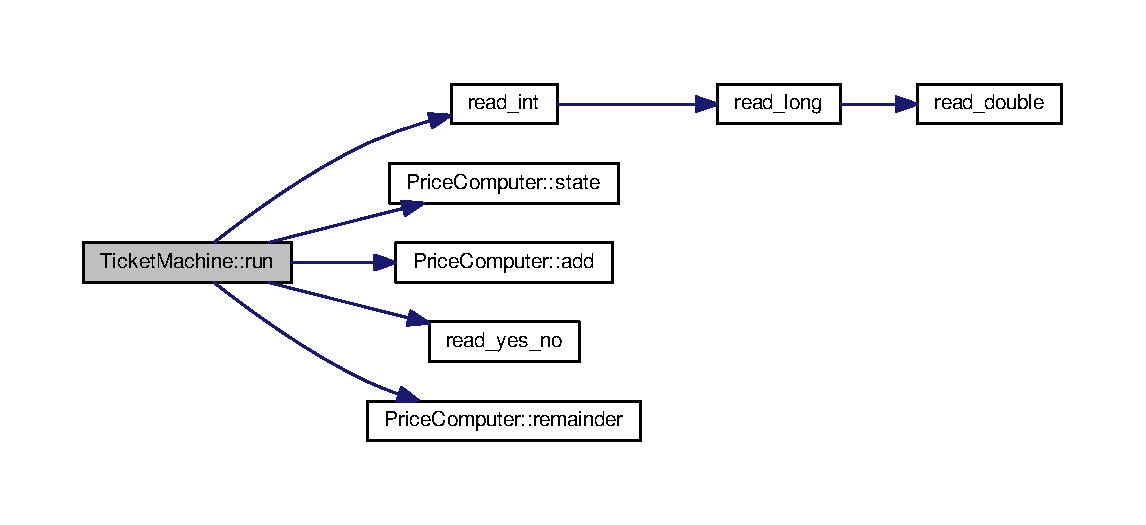
\includegraphics[width=350pt]{classTicketMachine_a8d68bde6ee1a9a5f08182df963c1b0a9_cgraph}
\end{center}
\end{figure}




The documentation for this class was generated from the following files\-:\begin{DoxyCompactItemize}
\item 
\hyperlink{ticket__machine_8h}{ticket\-\_\-machine.\-h}\item 
\hyperlink{ticket__machine_8cpp}{ticket\-\_\-machine.\-cpp}\end{DoxyCompactItemize}

\chapter{File Documentation}
\hypertarget{coin__slot_8cpp}{\section{coin\-\_\-slot.\-cpp File Reference}
\label{coin__slot_8cpp}\index{coin\-\_\-slot.\-cpp@{coin\-\_\-slot.\-cpp}}
}
{\ttfamily \#include $<$iostream$>$}\\*
{\ttfamily \#include $<$iomanip$>$}\\*
{\ttfamily \#include $<$sstream$>$}\\*
{\ttfamily \#include $<$vector$>$}\\*
{\ttfamily \#include $<$string$>$}\\*
{\ttfamily \#include $<$stdexcept$>$}\\*
{\ttfamily \#include \char`\"{}coin\-\_\-slot.\-h\char`\"{}}\\*
{\ttfamily \#include \char`\"{}console\-\_\-input.\-h\char`\"{}}\\*
Include dependency graph for coin\-\_\-slot.\-cpp\-:\nopagebreak
\begin{figure}[H]
\begin{center}
\leavevmode
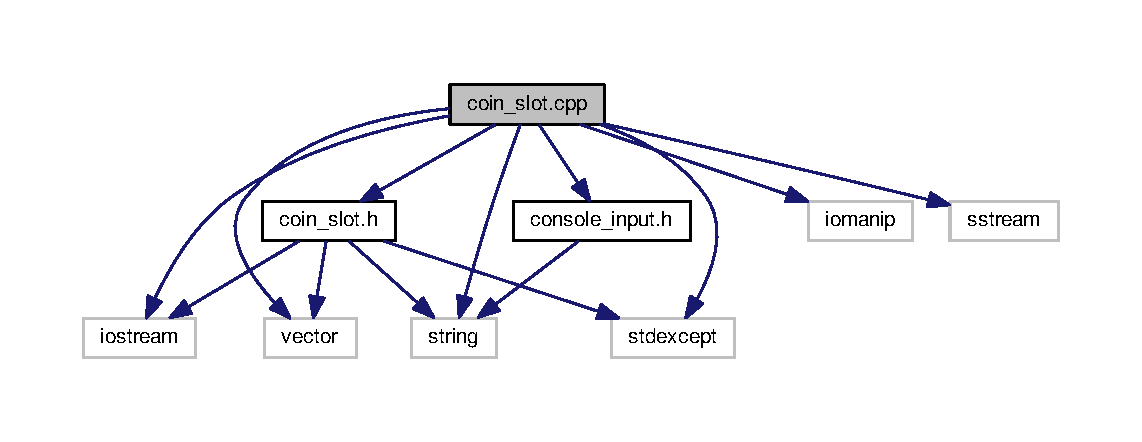
\includegraphics[width=350pt]{coin__slot_8cpp__incl}
\end{center}
\end{figure}
\subsection*{Functions}
\begin{DoxyCompactItemize}
\item 
istream \& \hyperlink{coin__slot_8cpp_a379e736965d39d908632dca531886f91}{operator$>$$>$} (istream \&input, \hyperlink{classCoinSlot}{Coin\-Slot} \&coin\-\_\-slot)
\item 
ostream \& \hyperlink{coin__slot_8cpp_aec2334964c7d0b94c15aaf9024c7c7d9}{operator$<$$<$} (ostream \&output, const \hyperlink{classCoinSlot}{Coin\-Slot} \&coin\-\_\-slot)
\end{DoxyCompactItemize}


\subsection{Function Documentation}
\hypertarget{coin__slot_8cpp_aec2334964c7d0b94c15aaf9024c7c7d9}{\index{coin\-\_\-slot.\-cpp@{coin\-\_\-slot.\-cpp}!operator$<$$<$@{operator$<$$<$}}
\index{operator$<$$<$@{operator$<$$<$}!coin_slot.cpp@{coin\-\_\-slot.\-cpp}}
\subsubsection[{operator$<$$<$}]{\setlength{\rightskip}{0pt plus 5cm}ostream\& operator$<$$<$ (
\begin{DoxyParamCaption}
\item[{ostream \&}]{output, }
\item[{const {\bf Coin\-Slot} \&}]{coin\-\_\-slot}
\end{DoxyParamCaption}
)}}\label{coin__slot_8cpp_aec2334964c7d0b94c15aaf9024c7c7d9}
Overrides the operator$<$$<$ \char`\"{}put to\char`\"{}. Handels standard string representation of a coin\-\_\-slot when \char`\"{}put to\char`\"{} an output stream.


\begin{DoxyParams}{Parameters}
{\em output} & io output stream. \\
\hline
{\em coin\-\_\-slot} & \hyperlink{classCoinSlot}{Coin\-Slot} to print to the output stream.\\
\hline
\end{DoxyParams}
\begin{DoxyReturn}{Returns}

\end{DoxyReturn}


Here is the call graph for this function\-:\nopagebreak
\begin{figure}[H]
\begin{center}
\leavevmode
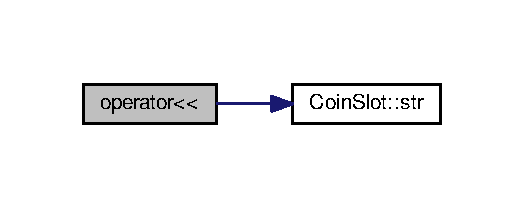
\includegraphics[width=252pt]{coin__slot_8cpp_aec2334964c7d0b94c15aaf9024c7c7d9_cgraph}
\end{center}
\end{figure}


\hypertarget{coin__slot_8cpp_a379e736965d39d908632dca531886f91}{\index{coin\-\_\-slot.\-cpp@{coin\-\_\-slot.\-cpp}!operator$>$$>$@{operator$>$$>$}}
\index{operator$>$$>$@{operator$>$$>$}!coin_slot.cpp@{coin\-\_\-slot.\-cpp}}
\subsubsection[{operator$>$$>$}]{\setlength{\rightskip}{0pt plus 5cm}istream\& operator$>$$>$ (
\begin{DoxyParamCaption}
\item[{istream \&}]{input, }
\item[{{\bf Coin\-Slot} \&}]{coin\-\_\-slot}
\end{DoxyParamCaption}
)}}\label{coin__slot_8cpp_a379e736965d39d908632dca531886f91}
Overrides the operator$>$$>$ \char`\"{}get from\char`\"{}. Handels the console input of a coin.


\begin{DoxyParams}{Parameters}
{\em input} & I\-O Input stream. \\
\hline
{\em coin\-\_\-slot} & \hyperlink{classCoinSlot}{Coin\-Slot} instance to insert a coin from the console.\\
\hline
\end{DoxyParams}
\begin{DoxyReturn}{Returns}
inputstream 
\end{DoxyReturn}


Here is the call graph for this function\-:\nopagebreak
\begin{figure}[H]
\begin{center}
\leavevmode
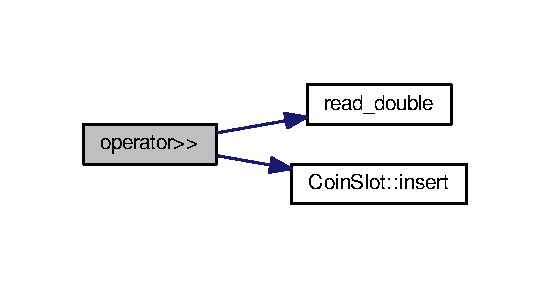
\includegraphics[width=264pt]{coin__slot_8cpp_a379e736965d39d908632dca531886f91_cgraph}
\end{center}
\end{figure}



\hypertarget{coin__slot_8h}{\section{coin\-\_\-slot.\-h File Reference}
\label{coin__slot_8h}\index{coin\-\_\-slot.\-h@{coin\-\_\-slot.\-h}}
}
{\ttfamily \#include $<$iostream$>$}\\*
{\ttfamily \#include $<$string$>$}\\*
{\ttfamily \#include $<$vector$>$}\\*
{\ttfamily \#include $<$stdexcept$>$}\\*
Include dependency graph for coin\-\_\-slot.\-h\-:\nopagebreak
\begin{figure}[H]
\begin{center}
\leavevmode
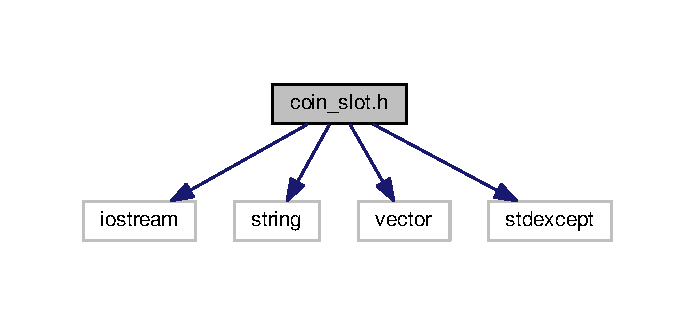
\includegraphics[width=333pt]{coin__slot_8h__incl}
\end{center}
\end{figure}
This graph shows which files directly or indirectly include this file\-:\nopagebreak
\begin{figure}[H]
\begin{center}
\leavevmode
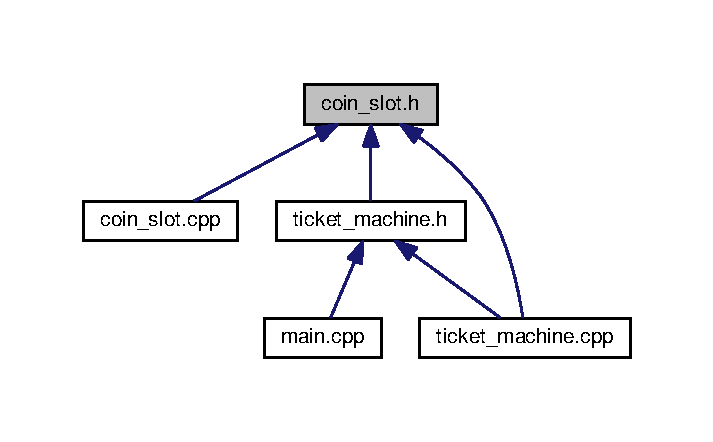
\includegraphics[width=342pt]{coin__slot_8h__dep__incl}
\end{center}
\end{figure}
\subsection*{Classes}
\begin{DoxyCompactItemize}
\item 
class \hyperlink{classCoinSlot}{Coin\-Slot}
\end{DoxyCompactItemize}
\subsection*{Functions}
\begin{DoxyCompactItemize}
\item 
istream \& \hyperlink{coin__slot_8h_a379e736965d39d908632dca531886f91}{operator$>$$>$} (istream \&input, \hyperlink{classCoinSlot}{Coin\-Slot} \&coin\-\_\-slot)
\item 
ostream \& \hyperlink{coin__slot_8h_aec2334964c7d0b94c15aaf9024c7c7d9}{operator$<$$<$} (ostream \&output, const \hyperlink{classCoinSlot}{Coin\-Slot} \&coin\-\_\-slot)
\end{DoxyCompactItemize}


\subsection{Function Documentation}
\hypertarget{coin__slot_8h_aec2334964c7d0b94c15aaf9024c7c7d9}{\index{coin\-\_\-slot.\-h@{coin\-\_\-slot.\-h}!operator$<$$<$@{operator$<$$<$}}
\index{operator$<$$<$@{operator$<$$<$}!coin_slot.h@{coin\-\_\-slot.\-h}}
\subsubsection[{operator$<$$<$}]{\setlength{\rightskip}{0pt plus 5cm}ostream\& operator$<$$<$ (
\begin{DoxyParamCaption}
\item[{ostream \&}]{output, }
\item[{const {\bf Coin\-Slot} \&}]{coin\-\_\-slot}
\end{DoxyParamCaption}
)}}\label{coin__slot_8h_aec2334964c7d0b94c15aaf9024c7c7d9}
Overrides the operator$<$$<$ \char`\"{}put to\char`\"{}. Handels standard string representation of a coin\-\_\-slot when \char`\"{}put to\char`\"{} an output stream.


\begin{DoxyParams}{Parameters}
{\em output} & io output stream. \\
\hline
{\em coin\-\_\-slot} & \hyperlink{classCoinSlot}{Coin\-Slot} to print to the output stream.\\
\hline
\end{DoxyParams}
\begin{DoxyReturn}{Returns}

\end{DoxyReturn}


Here is the call graph for this function\-:\nopagebreak
\begin{figure}[H]
\begin{center}
\leavevmode
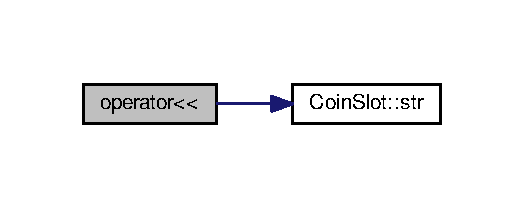
\includegraphics[width=252pt]{coin__slot_8h_aec2334964c7d0b94c15aaf9024c7c7d9_cgraph}
\end{center}
\end{figure}


\hypertarget{coin__slot_8h_a379e736965d39d908632dca531886f91}{\index{coin\-\_\-slot.\-h@{coin\-\_\-slot.\-h}!operator$>$$>$@{operator$>$$>$}}
\index{operator$>$$>$@{operator$>$$>$}!coin_slot.h@{coin\-\_\-slot.\-h}}
\subsubsection[{operator$>$$>$}]{\setlength{\rightskip}{0pt plus 5cm}istream\& operator$>$$>$ (
\begin{DoxyParamCaption}
\item[{istream \&}]{input, }
\item[{{\bf Coin\-Slot} \&}]{coin\-\_\-slot}
\end{DoxyParamCaption}
)}}\label{coin__slot_8h_a379e736965d39d908632dca531886f91}
Overrides the operator$>$$>$ \char`\"{}get from\char`\"{}. Handels the console input of a coin.


\begin{DoxyParams}{Parameters}
{\em input} & I\-O Input stream. \\
\hline
{\em coin\-\_\-slot} & \hyperlink{classCoinSlot}{Coin\-Slot} instance to insert a coin from the console.\\
\hline
\end{DoxyParams}
\begin{DoxyReturn}{Returns}
inputstream 
\end{DoxyReturn}


Here is the call graph for this function\-:\nopagebreak
\begin{figure}[H]
\begin{center}
\leavevmode
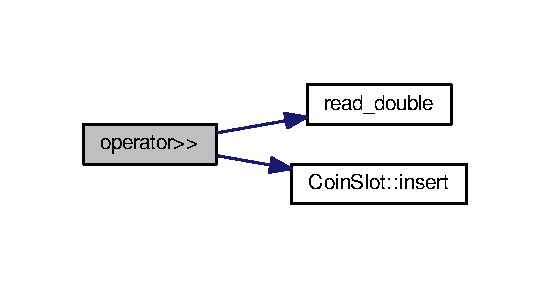
\includegraphics[width=264pt]{coin__slot_8h_a379e736965d39d908632dca531886f91_cgraph}
\end{center}
\end{figure}



\hypertarget{console__input_8cpp}{\section{console\-\_\-input.\-cpp File Reference}
\label{console__input_8cpp}\index{console\-\_\-input.\-cpp@{console\-\_\-input.\-cpp}}
}
{\ttfamily \#include $<$iostream$>$}\\*
{\ttfamily \#include $<$limits$>$}\\*
{\ttfamily \#include $<$string$>$}\\*
{\ttfamily \#include \char`\"{}console\-\_\-input.\-h\char`\"{}}\\*
Include dependency graph for console\-\_\-input.\-cpp\-:\nopagebreak
\begin{figure}[H]
\begin{center}
\leavevmode
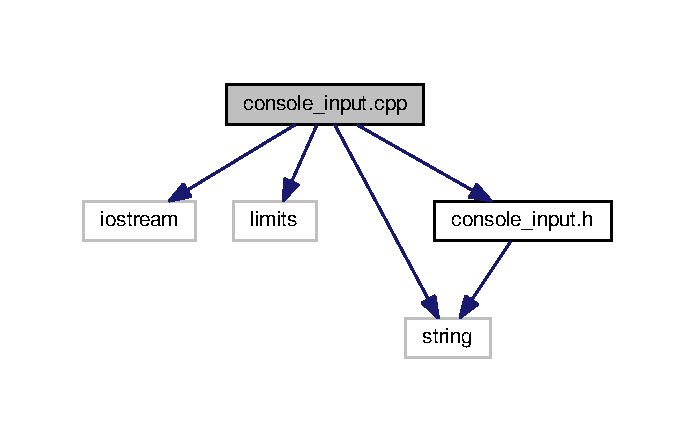
\includegraphics[width=332pt]{console__input_8cpp__incl}
\end{center}
\end{figure}
\subsection*{Functions}
\begin{DoxyCompactItemize}
\item 
double \hyperlink{console__input_8cpp_a8a9df77c5c4adba7ebadb77f3b3dc8ee}{read\-\_\-double} (double min, double max)
\item 
double \hyperlink{console__input_8cpp_a65f2421973540c10e5ae7d10177c566a}{read\-\_\-double} ()
\item 
double \hyperlink{console__input_8cpp_a46878a8594ba71f54911c572031d4614}{read\-\_\-double} (string text)
\item 
double \hyperlink{console__input_8cpp_aca43573be8fe10d4bfede3fc5bd0bd63}{read\-\_\-double} (string text, double min, double max)
\item 
long \hyperlink{console__input_8cpp_a710a686867142de265860584f4147592}{read\-\_\-long} (long min, long max)
\item 
long \hyperlink{console__input_8cpp_a347c616893b725a74f60ea1f7ee325d2}{read\-\_\-long} ()
\item 
long \hyperlink{console__input_8cpp_a9128c63513d87af5259597d8c9930476}{read\-\_\-long} (string text)
\item 
long \hyperlink{console__input_8cpp_a03ebbd2a45117ee03be4e9002210ab36}{read\-\_\-long} (string text, long min, long max)
\item 
int \hyperlink{console__input_8cpp_ad0ccfbb50d0e333ef8acfeab2b7d8071}{read\-\_\-int} (int min, int max)
\item 
int \hyperlink{console__input_8cpp_af310540093ee953c3018bc13bbde3da5}{read\-\_\-int} ()
\item 
int \hyperlink{console__input_8cpp_aaaf3786f6b4803f3120609011de4b0db}{read\-\_\-int} (string text)
\item 
int \hyperlink{console__input_8cpp_a4f8c1bb51d432116d3eda43db3340c8c}{read\-\_\-int} (string text, int min, int max)
\item 
bool \hyperlink{console__input_8cpp_a6bac3909a28fff2736a171022343380b}{read\-\_\-yes\-\_\-no} (string text)
\item 
string \hyperlink{console__input_8cpp_a44ccadd65be527f89bdcf6d27a3b1147}{read\-\_\-text} (string text)
\end{DoxyCompactItemize}


\subsection{Function Documentation}
\hypertarget{console__input_8cpp_a8a9df77c5c4adba7ebadb77f3b3dc8ee}{\index{console\-\_\-input.\-cpp@{console\-\_\-input.\-cpp}!read\-\_\-double@{read\-\_\-double}}
\index{read\-\_\-double@{read\-\_\-double}!console_input.cpp@{console\-\_\-input.\-cpp}}
\subsubsection[{read\-\_\-double}]{\setlength{\rightskip}{0pt plus 5cm}double read\-\_\-double (
\begin{DoxyParamCaption}
\item[{double}]{min, }
\item[{double}]{max}
\end{DoxyParamCaption}
)}}\label{console__input_8cpp_a8a9df77c5c4adba7ebadb77f3b3dc8ee}
Reads a double value in between a given interval from the console. When the entered value is not valid to the interval, the user gets prompted to reenter a valid.


\begin{DoxyParams}{Parameters}
{\em min} & lower bound of the interval. \\
\hline
{\em max} & top bound of the interval\\
\hline
\end{DoxyParams}
\begin{DoxyReturn}{Returns}
a double value in between min and max. 
\end{DoxyReturn}
\hypertarget{console__input_8cpp_a65f2421973540c10e5ae7d10177c566a}{\index{console\-\_\-input.\-cpp@{console\-\_\-input.\-cpp}!read\-\_\-double@{read\-\_\-double}}
\index{read\-\_\-double@{read\-\_\-double}!console_input.cpp@{console\-\_\-input.\-cpp}}
\subsubsection[{read\-\_\-double}]{\setlength{\rightskip}{0pt plus 5cm}double read\-\_\-double (
\begin{DoxyParamCaption}
{}
\end{DoxyParamCaption}
)}}\label{console__input_8cpp_a65f2421973540c10e5ae7d10177c566a}
Reads a double value from the console in between the whole range of double.

\begin{DoxyReturn}{Returns}
a valid double value. 
\end{DoxyReturn}


Here is the call graph for this function\-:\nopagebreak
\begin{figure}[H]
\begin{center}
\leavevmode
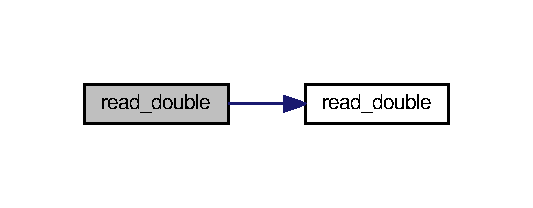
\includegraphics[width=256pt]{console__input_8cpp_a65f2421973540c10e5ae7d10177c566a_cgraph}
\end{center}
\end{figure}


\hypertarget{console__input_8cpp_a46878a8594ba71f54911c572031d4614}{\index{console\-\_\-input.\-cpp@{console\-\_\-input.\-cpp}!read\-\_\-double@{read\-\_\-double}}
\index{read\-\_\-double@{read\-\_\-double}!console_input.cpp@{console\-\_\-input.\-cpp}}
\subsubsection[{read\-\_\-double}]{\setlength{\rightskip}{0pt plus 5cm}double read\-\_\-double (
\begin{DoxyParamCaption}
\item[{string}]{text}
\end{DoxyParamCaption}
)}}\label{console__input_8cpp_a46878a8594ba71f54911c572031d4614}
Prints a text to the console and reads a double value from the console in between the whole range of double.


\begin{DoxyParams}{Parameters}
{\em text} & text to print to the console.\\
\hline
\end{DoxyParams}
\begin{DoxyReturn}{Returns}
a valid double value. 
\end{DoxyReturn}


Here is the call graph for this function\-:\nopagebreak
\begin{figure}[H]
\begin{center}
\leavevmode
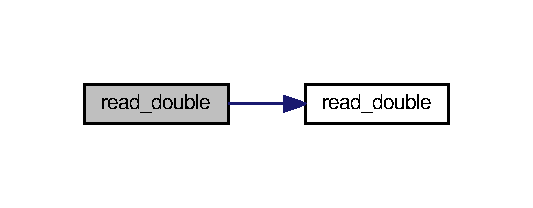
\includegraphics[width=256pt]{console__input_8cpp_a46878a8594ba71f54911c572031d4614_cgraph}
\end{center}
\end{figure}


\hypertarget{console__input_8cpp_aca43573be8fe10d4bfede3fc5bd0bd63}{\index{console\-\_\-input.\-cpp@{console\-\_\-input.\-cpp}!read\-\_\-double@{read\-\_\-double}}
\index{read\-\_\-double@{read\-\_\-double}!console_input.cpp@{console\-\_\-input.\-cpp}}
\subsubsection[{read\-\_\-double}]{\setlength{\rightskip}{0pt plus 5cm}double read\-\_\-double (
\begin{DoxyParamCaption}
\item[{string}]{text, }
\item[{double}]{min, }
\item[{double}]{max}
\end{DoxyParamCaption}
)}}\label{console__input_8cpp_aca43573be8fe10d4bfede3fc5bd0bd63}


Here is the call graph for this function\-:\nopagebreak
\begin{figure}[H]
\begin{center}
\leavevmode
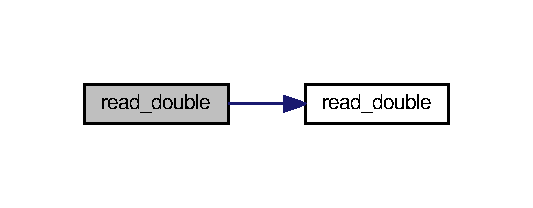
\includegraphics[width=256pt]{console__input_8cpp_aca43573be8fe10d4bfede3fc5bd0bd63_cgraph}
\end{center}
\end{figure}


\hypertarget{console__input_8cpp_ad0ccfbb50d0e333ef8acfeab2b7d8071}{\index{console\-\_\-input.\-cpp@{console\-\_\-input.\-cpp}!read\-\_\-int@{read\-\_\-int}}
\index{read\-\_\-int@{read\-\_\-int}!console_input.cpp@{console\-\_\-input.\-cpp}}
\subsubsection[{read\-\_\-int}]{\setlength{\rightskip}{0pt plus 5cm}int read\-\_\-int (
\begin{DoxyParamCaption}
\item[{int}]{min, }
\item[{int}]{max}
\end{DoxyParamCaption}
)}}\label{console__input_8cpp_ad0ccfbb50d0e333ef8acfeab2b7d8071}
Reads a integer value in between a given interval from the console. When the entered value is not valid to the interval, the user gets prompted to reenter a valid.


\begin{DoxyParams}{Parameters}
{\em min} & lower bound of the interval. \\
\hline
{\em max} & top bound of the interval\\
\hline
\end{DoxyParams}
\begin{DoxyReturn}{Returns}
a int value in between min and max. 
\end{DoxyReturn}


Here is the call graph for this function\-:\nopagebreak
\begin{figure}[H]
\begin{center}
\leavevmode
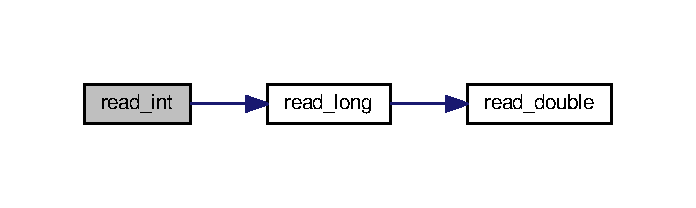
\includegraphics[width=334pt]{console__input_8cpp_ad0ccfbb50d0e333ef8acfeab2b7d8071_cgraph}
\end{center}
\end{figure}


\hypertarget{console__input_8cpp_af310540093ee953c3018bc13bbde3da5}{\index{console\-\_\-input.\-cpp@{console\-\_\-input.\-cpp}!read\-\_\-int@{read\-\_\-int}}
\index{read\-\_\-int@{read\-\_\-int}!console_input.cpp@{console\-\_\-input.\-cpp}}
\subsubsection[{read\-\_\-int}]{\setlength{\rightskip}{0pt plus 5cm}int read\-\_\-int (
\begin{DoxyParamCaption}
{}
\end{DoxyParamCaption}
)}}\label{console__input_8cpp_af310540093ee953c3018bc13bbde3da5}
Reads an integer value from the terminal in between the whole range of long.

\begin{DoxyReturn}{Returns}
a valid integer value. 
\end{DoxyReturn}


Here is the call graph for this function\-:\nopagebreak
\begin{figure}[H]
\begin{center}
\leavevmode
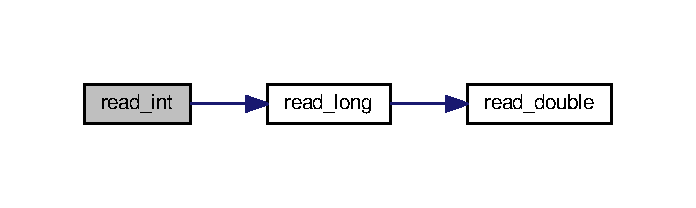
\includegraphics[width=334pt]{console__input_8cpp_af310540093ee953c3018bc13bbde3da5_cgraph}
\end{center}
\end{figure}


\hypertarget{console__input_8cpp_aaaf3786f6b4803f3120609011de4b0db}{\index{console\-\_\-input.\-cpp@{console\-\_\-input.\-cpp}!read\-\_\-int@{read\-\_\-int}}
\index{read\-\_\-int@{read\-\_\-int}!console_input.cpp@{console\-\_\-input.\-cpp}}
\subsubsection[{read\-\_\-int}]{\setlength{\rightskip}{0pt plus 5cm}int read\-\_\-int (
\begin{DoxyParamCaption}
\item[{string}]{text}
\end{DoxyParamCaption}
)}}\label{console__input_8cpp_aaaf3786f6b4803f3120609011de4b0db}
Prints a text to the console and reads a integer value from the console in between the whole range of integer.


\begin{DoxyParams}{Parameters}
{\em text} & text to print to the console.\\
\hline
\end{DoxyParams}
\begin{DoxyReturn}{Returns}
a valid integer value. 
\end{DoxyReturn}


Here is the call graph for this function\-:\nopagebreak
\begin{figure}[H]
\begin{center}
\leavevmode
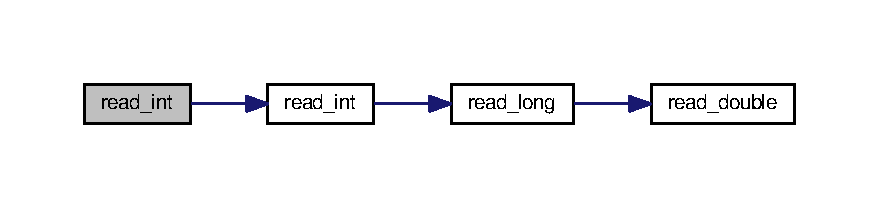
\includegraphics[width=350pt]{console__input_8cpp_aaaf3786f6b4803f3120609011de4b0db_cgraph}
\end{center}
\end{figure}


\hypertarget{console__input_8cpp_a4f8c1bb51d432116d3eda43db3340c8c}{\index{console\-\_\-input.\-cpp@{console\-\_\-input.\-cpp}!read\-\_\-int@{read\-\_\-int}}
\index{read\-\_\-int@{read\-\_\-int}!console_input.cpp@{console\-\_\-input.\-cpp}}
\subsubsection[{read\-\_\-int}]{\setlength{\rightskip}{0pt plus 5cm}int read\-\_\-int (
\begin{DoxyParamCaption}
\item[{string}]{text, }
\item[{int}]{min, }
\item[{int}]{max}
\end{DoxyParamCaption}
)}}\label{console__input_8cpp_a4f8c1bb51d432116d3eda43db3340c8c}
Prints a text to the console and reads a integer value in between a given interval from the console. When the value is not in between the interval, the user gets prompted to reeinter a valid value.


\begin{DoxyParams}{Parameters}
{\em text} & text to print to the console. \\
\hline
{\em min} & lower bound of the interval. \\
\hline
{\em max} & top bound of the interval.\\
\hline
\end{DoxyParams}
\begin{DoxyReturn}{Returns}
a integer value in between min and max. 
\end{DoxyReturn}


Here is the call graph for this function\-:\nopagebreak
\begin{figure}[H]
\begin{center}
\leavevmode
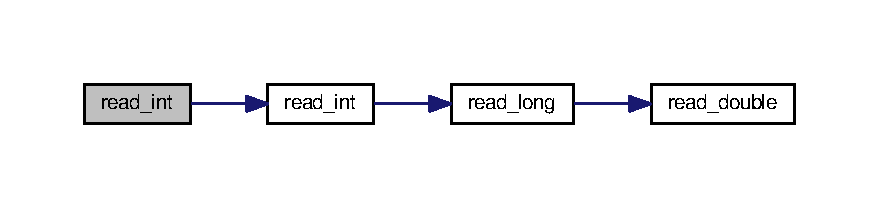
\includegraphics[width=350pt]{console__input_8cpp_a4f8c1bb51d432116d3eda43db3340c8c_cgraph}
\end{center}
\end{figure}


\hypertarget{console__input_8cpp_a710a686867142de265860584f4147592}{\index{console\-\_\-input.\-cpp@{console\-\_\-input.\-cpp}!read\-\_\-long@{read\-\_\-long}}
\index{read\-\_\-long@{read\-\_\-long}!console_input.cpp@{console\-\_\-input.\-cpp}}
\subsubsection[{read\-\_\-long}]{\setlength{\rightskip}{0pt plus 5cm}long read\-\_\-long (
\begin{DoxyParamCaption}
\item[{long}]{min, }
\item[{long}]{max}
\end{DoxyParamCaption}
)}}\label{console__input_8cpp_a710a686867142de265860584f4147592}
Reads a long value in between a given interval from the console. When the entered value is not valid to the interval, the user gets prompted to reenter a valid.


\begin{DoxyParams}{Parameters}
{\em min} & lower bound of the interval. \\
\hline
{\em max} & top bound of the interval\\
\hline
\end{DoxyParams}
\begin{DoxyReturn}{Returns}
a long value in between min and max. 
\end{DoxyReturn}


Here is the call graph for this function\-:\nopagebreak
\begin{figure}[H]
\begin{center}
\leavevmode
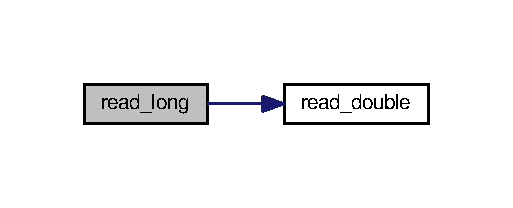
\includegraphics[width=246pt]{console__input_8cpp_a710a686867142de265860584f4147592_cgraph}
\end{center}
\end{figure}


\hypertarget{console__input_8cpp_a347c616893b725a74f60ea1f7ee325d2}{\index{console\-\_\-input.\-cpp@{console\-\_\-input.\-cpp}!read\-\_\-long@{read\-\_\-long}}
\index{read\-\_\-long@{read\-\_\-long}!console_input.cpp@{console\-\_\-input.\-cpp}}
\subsubsection[{read\-\_\-long}]{\setlength{\rightskip}{0pt plus 5cm}long read\-\_\-long (
\begin{DoxyParamCaption}
{}
\end{DoxyParamCaption}
)}}\label{console__input_8cpp_a347c616893b725a74f60ea1f7ee325d2}
Reads a long value from the terminal in between the whole range of long.

\begin{DoxyReturn}{Returns}
a valid long value. 
\end{DoxyReturn}


Here is the call graph for this function\-:\nopagebreak
\begin{figure}[H]
\begin{center}
\leavevmode
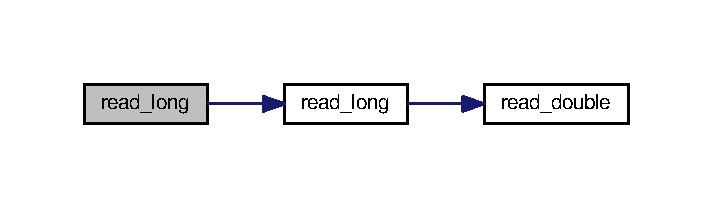
\includegraphics[width=342pt]{console__input_8cpp_a347c616893b725a74f60ea1f7ee325d2_cgraph}
\end{center}
\end{figure}


\hypertarget{console__input_8cpp_a9128c63513d87af5259597d8c9930476}{\index{console\-\_\-input.\-cpp@{console\-\_\-input.\-cpp}!read\-\_\-long@{read\-\_\-long}}
\index{read\-\_\-long@{read\-\_\-long}!console_input.cpp@{console\-\_\-input.\-cpp}}
\subsubsection[{read\-\_\-long}]{\setlength{\rightskip}{0pt plus 5cm}long read\-\_\-long (
\begin{DoxyParamCaption}
\item[{string}]{text}
\end{DoxyParamCaption}
)}}\label{console__input_8cpp_a9128c63513d87af5259597d8c9930476}
Prints a text to the console and reads a long value from the console in between the whole range of long.


\begin{DoxyParams}{Parameters}
{\em text} & text to print to the console.\\
\hline
\end{DoxyParams}
\begin{DoxyReturn}{Returns}
a valid long value. 
\end{DoxyReturn}


Here is the call graph for this function\-:\nopagebreak
\begin{figure}[H]
\begin{center}
\leavevmode
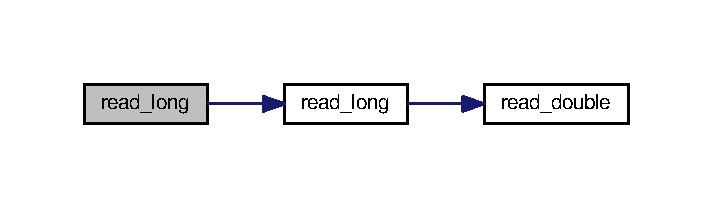
\includegraphics[width=342pt]{console__input_8cpp_a9128c63513d87af5259597d8c9930476_cgraph}
\end{center}
\end{figure}


\hypertarget{console__input_8cpp_a03ebbd2a45117ee03be4e9002210ab36}{\index{console\-\_\-input.\-cpp@{console\-\_\-input.\-cpp}!read\-\_\-long@{read\-\_\-long}}
\index{read\-\_\-long@{read\-\_\-long}!console_input.cpp@{console\-\_\-input.\-cpp}}
\subsubsection[{read\-\_\-long}]{\setlength{\rightskip}{0pt plus 5cm}long read\-\_\-long (
\begin{DoxyParamCaption}
\item[{string}]{text, }
\item[{long}]{min, }
\item[{long}]{max}
\end{DoxyParamCaption}
)}}\label{console__input_8cpp_a03ebbd2a45117ee03be4e9002210ab36}
Prints a text to the console and reads a long value in between a given interval from the console. When the value is not in between the interval, the user gets prompted to reeinter a valid value.


\begin{DoxyParams}{Parameters}
{\em text} & text to print to the console. \\
\hline
{\em min} & lower bound of the interval. \\
\hline
{\em max} & top bound of the interval.\\
\hline
\end{DoxyParams}
\begin{DoxyReturn}{Returns}
a long value in between min and max. 
\end{DoxyReturn}


Here is the call graph for this function\-:\nopagebreak
\begin{figure}[H]
\begin{center}
\leavevmode
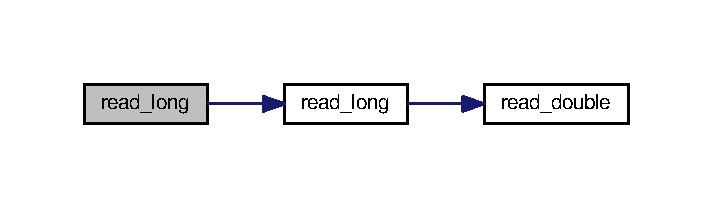
\includegraphics[width=342pt]{console__input_8cpp_a03ebbd2a45117ee03be4e9002210ab36_cgraph}
\end{center}
\end{figure}


\hypertarget{console__input_8cpp_a44ccadd65be527f89bdcf6d27a3b1147}{\index{console\-\_\-input.\-cpp@{console\-\_\-input.\-cpp}!read\-\_\-text@{read\-\_\-text}}
\index{read\-\_\-text@{read\-\_\-text}!console_input.cpp@{console\-\_\-input.\-cpp}}
\subsubsection[{read\-\_\-text}]{\setlength{\rightskip}{0pt plus 5cm}string read\-\_\-text (
\begin{DoxyParamCaption}
\item[{string}]{text}
\end{DoxyParamCaption}
)}}\label{console__input_8cpp_a44ccadd65be527f89bdcf6d27a3b1147}
\hypertarget{console__input_8cpp_a6bac3909a28fff2736a171022343380b}{\index{console\-\_\-input.\-cpp@{console\-\_\-input.\-cpp}!read\-\_\-yes\-\_\-no@{read\-\_\-yes\-\_\-no}}
\index{read\-\_\-yes\-\_\-no@{read\-\_\-yes\-\_\-no}!console_input.cpp@{console\-\_\-input.\-cpp}}
\subsubsection[{read\-\_\-yes\-\_\-no}]{\setlength{\rightskip}{0pt plus 5cm}bool read\-\_\-yes\-\_\-no (
\begin{DoxyParamCaption}
\item[{string}]{text}
\end{DoxyParamCaption}
)}}\label{console__input_8cpp_a6bac3909a28fff2736a171022343380b}

\hypertarget{console__input_8h}{\section{console\-\_\-input.\-h File Reference}
\label{console__input_8h}\index{console\-\_\-input.\-h@{console\-\_\-input.\-h}}
}
{\ttfamily \#include $<$string$>$}\\*
Include dependency graph for console\-\_\-input.\-h\-:\nopagebreak
\begin{figure}[H]
\begin{center}
\leavevmode
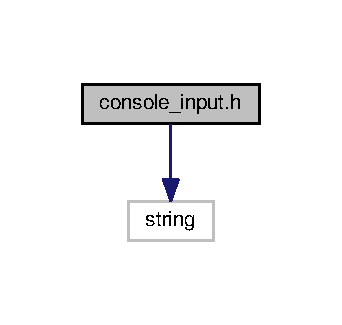
\includegraphics[width=164pt]{console__input_8h__incl}
\end{center}
\end{figure}
This graph shows which files directly or indirectly include this file\-:\nopagebreak
\begin{figure}[H]
\begin{center}
\leavevmode
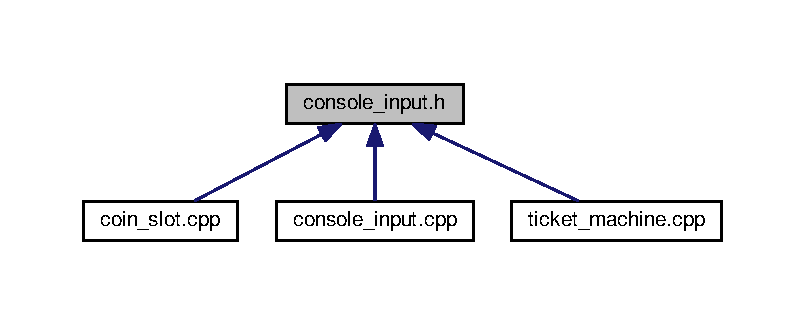
\includegraphics[width=264pt]{console__input_8h__dep__incl}
\end{center}
\end{figure}
\subsection*{Functions}
\begin{DoxyCompactItemize}
\item 
double \hyperlink{console__input_8h_a8a9df77c5c4adba7ebadb77f3b3dc8ee}{read\-\_\-double} (double min, double max)
\item 
double \hyperlink{console__input_8h_a46878a8594ba71f54911c572031d4614}{read\-\_\-double} (string text)
\item 
double \hyperlink{console__input_8h_aca43573be8fe10d4bfede3fc5bd0bd63}{read\-\_\-double} (string text, double min, double max)
\item 
double \hyperlink{console__input_8h_a65f2421973540c10e5ae7d10177c566a}{read\-\_\-double} ()
\item 
void \hyperlink{console__input_8h_afc6e4adf69aec96a5eae4249fbbc7201}{read\-\_\-enter} ()
\item 
long \hyperlink{console__input_8h_a03ebbd2a45117ee03be4e9002210ab36}{read\-\_\-long} (string text, long min, long max)
\item 
long \hyperlink{console__input_8h_a710a686867142de265860584f4147592}{read\-\_\-long} (long min, long max)
\item 
long \hyperlink{console__input_8h_a9128c63513d87af5259597d8c9930476}{read\-\_\-long} (string text)
\item 
long \hyperlink{console__input_8h_a347c616893b725a74f60ea1f7ee325d2}{read\-\_\-long} ()
\item 
int \hyperlink{console__input_8h_a4f8c1bb51d432116d3eda43db3340c8c}{read\-\_\-int} (string text, int min, int max)
\item 
int \hyperlink{console__input_8h_ad0ccfbb50d0e333ef8acfeab2b7d8071}{read\-\_\-int} (int min, int max)
\item 
int \hyperlink{console__input_8h_aaaf3786f6b4803f3120609011de4b0db}{read\-\_\-int} (string text)
\item 
int \hyperlink{console__input_8h_af310540093ee953c3018bc13bbde3da5}{read\-\_\-int} ()
\item 
bool \hyperlink{console__input_8h_a6bac3909a28fff2736a171022343380b}{read\-\_\-yes\-\_\-no} (string text)
\item 
string \hyperlink{console__input_8h_a44ccadd65be527f89bdcf6d27a3b1147}{read\-\_\-text} (string text)
\end{DoxyCompactItemize}


\subsection{Function Documentation}
\hypertarget{console__input_8h_a8a9df77c5c4adba7ebadb77f3b3dc8ee}{\index{console\-\_\-input.\-h@{console\-\_\-input.\-h}!read\-\_\-double@{read\-\_\-double}}
\index{read\-\_\-double@{read\-\_\-double}!console_input.h@{console\-\_\-input.\-h}}
\subsubsection[{read\-\_\-double}]{\setlength{\rightskip}{0pt plus 5cm}double read\-\_\-double (
\begin{DoxyParamCaption}
\item[{double}]{min, }
\item[{double}]{max}
\end{DoxyParamCaption}
)}}\label{console__input_8h_a8a9df77c5c4adba7ebadb77f3b3dc8ee}
Reads a double value in between a given interval from the console. When the entered value is not valid to the interval, the user gets prompted to reenter a valid.


\begin{DoxyParams}{Parameters}
{\em min} & lower bound of the interval. \\
\hline
{\em max} & top bound of the interval\\
\hline
\end{DoxyParams}
\begin{DoxyReturn}{Returns}
a double value in between min and max. 
\end{DoxyReturn}
\hypertarget{console__input_8h_a46878a8594ba71f54911c572031d4614}{\index{console\-\_\-input.\-h@{console\-\_\-input.\-h}!read\-\_\-double@{read\-\_\-double}}
\index{read\-\_\-double@{read\-\_\-double}!console_input.h@{console\-\_\-input.\-h}}
\subsubsection[{read\-\_\-double}]{\setlength{\rightskip}{0pt plus 5cm}double read\-\_\-double (
\begin{DoxyParamCaption}
\item[{string}]{text}
\end{DoxyParamCaption}
)}}\label{console__input_8h_a46878a8594ba71f54911c572031d4614}
Prints a text to the console and reads a double value from the console in between the whole range of double.


\begin{DoxyParams}{Parameters}
{\em text} & text to print to the console.\\
\hline
\end{DoxyParams}
\begin{DoxyReturn}{Returns}
a valid double value. 
\end{DoxyReturn}


Here is the call graph for this function\-:\nopagebreak
\begin{figure}[H]
\begin{center}
\leavevmode
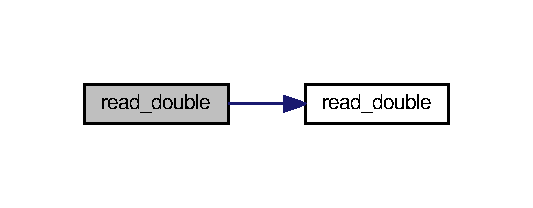
\includegraphics[width=256pt]{console__input_8h_a46878a8594ba71f54911c572031d4614_cgraph}
\end{center}
\end{figure}


\hypertarget{console__input_8h_aca43573be8fe10d4bfede3fc5bd0bd63}{\index{console\-\_\-input.\-h@{console\-\_\-input.\-h}!read\-\_\-double@{read\-\_\-double}}
\index{read\-\_\-double@{read\-\_\-double}!console_input.h@{console\-\_\-input.\-h}}
\subsubsection[{read\-\_\-double}]{\setlength{\rightskip}{0pt plus 5cm}double read\-\_\-double (
\begin{DoxyParamCaption}
\item[{string}]{text, }
\item[{double}]{min, }
\item[{double}]{max}
\end{DoxyParamCaption}
)}}\label{console__input_8h_aca43573be8fe10d4bfede3fc5bd0bd63}


Here is the call graph for this function\-:\nopagebreak
\begin{figure}[H]
\begin{center}
\leavevmode
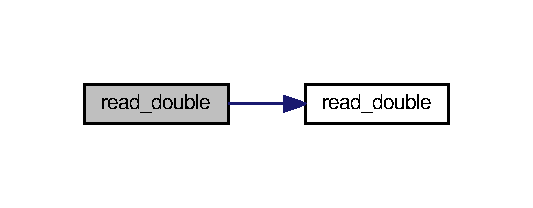
\includegraphics[width=256pt]{console__input_8h_aca43573be8fe10d4bfede3fc5bd0bd63_cgraph}
\end{center}
\end{figure}


\hypertarget{console__input_8h_a65f2421973540c10e5ae7d10177c566a}{\index{console\-\_\-input.\-h@{console\-\_\-input.\-h}!read\-\_\-double@{read\-\_\-double}}
\index{read\-\_\-double@{read\-\_\-double}!console_input.h@{console\-\_\-input.\-h}}
\subsubsection[{read\-\_\-double}]{\setlength{\rightskip}{0pt plus 5cm}double read\-\_\-double (
\begin{DoxyParamCaption}
{}
\end{DoxyParamCaption}
)}}\label{console__input_8h_a65f2421973540c10e5ae7d10177c566a}
Reads a double value from the console in between the whole range of double.

\begin{DoxyReturn}{Returns}
a valid double value. 
\end{DoxyReturn}


Here is the call graph for this function\-:\nopagebreak
\begin{figure}[H]
\begin{center}
\leavevmode
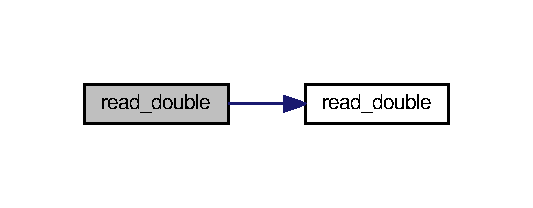
\includegraphics[width=256pt]{console__input_8h_a65f2421973540c10e5ae7d10177c566a_cgraph}
\end{center}
\end{figure}


\hypertarget{console__input_8h_afc6e4adf69aec96a5eae4249fbbc7201}{\index{console\-\_\-input.\-h@{console\-\_\-input.\-h}!read\-\_\-enter@{read\-\_\-enter}}
\index{read\-\_\-enter@{read\-\_\-enter}!console_input.h@{console\-\_\-input.\-h}}
\subsubsection[{read\-\_\-enter}]{\setlength{\rightskip}{0pt plus 5cm}void read\-\_\-enter (
\begin{DoxyParamCaption}
{}
\end{DoxyParamCaption}
)}}\label{console__input_8h_afc6e4adf69aec96a5eae4249fbbc7201}
\hypertarget{console__input_8h_a4f8c1bb51d432116d3eda43db3340c8c}{\index{console\-\_\-input.\-h@{console\-\_\-input.\-h}!read\-\_\-int@{read\-\_\-int}}
\index{read\-\_\-int@{read\-\_\-int}!console_input.h@{console\-\_\-input.\-h}}
\subsubsection[{read\-\_\-int}]{\setlength{\rightskip}{0pt plus 5cm}int read\-\_\-int (
\begin{DoxyParamCaption}
\item[{string}]{text, }
\item[{int}]{min, }
\item[{int}]{max}
\end{DoxyParamCaption}
)}}\label{console__input_8h_a4f8c1bb51d432116d3eda43db3340c8c}
Prints a text to the console and reads a integer value in between a given interval from the console. When the value is not in between the interval, the user gets prompted to reeinter a valid value.


\begin{DoxyParams}{Parameters}
{\em text} & text to print to the console. \\
\hline
{\em min} & lower bound of the interval. \\
\hline
{\em max} & top bound of the interval.\\
\hline
\end{DoxyParams}
\begin{DoxyReturn}{Returns}
a integer value in between min and max. 
\end{DoxyReturn}


Here is the call graph for this function\-:\nopagebreak
\begin{figure}[H]
\begin{center}
\leavevmode
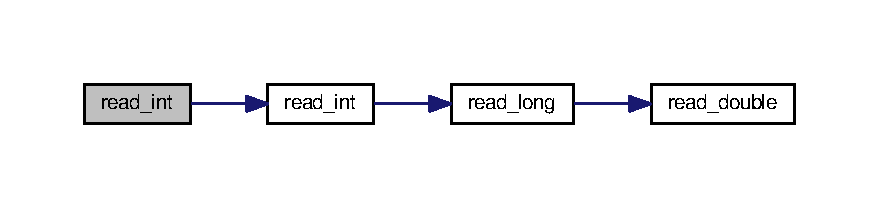
\includegraphics[width=350pt]{console__input_8h_a4f8c1bb51d432116d3eda43db3340c8c_cgraph}
\end{center}
\end{figure}


\hypertarget{console__input_8h_ad0ccfbb50d0e333ef8acfeab2b7d8071}{\index{console\-\_\-input.\-h@{console\-\_\-input.\-h}!read\-\_\-int@{read\-\_\-int}}
\index{read\-\_\-int@{read\-\_\-int}!console_input.h@{console\-\_\-input.\-h}}
\subsubsection[{read\-\_\-int}]{\setlength{\rightskip}{0pt plus 5cm}int read\-\_\-int (
\begin{DoxyParamCaption}
\item[{int}]{min, }
\item[{int}]{max}
\end{DoxyParamCaption}
)}}\label{console__input_8h_ad0ccfbb50d0e333ef8acfeab2b7d8071}
Reads a integer value in between a given interval from the console. When the entered value is not valid to the interval, the user gets prompted to reenter a valid.


\begin{DoxyParams}{Parameters}
{\em min} & lower bound of the interval. \\
\hline
{\em max} & top bound of the interval\\
\hline
\end{DoxyParams}
\begin{DoxyReturn}{Returns}
a int value in between min and max. 
\end{DoxyReturn}


Here is the call graph for this function\-:\nopagebreak
\begin{figure}[H]
\begin{center}
\leavevmode
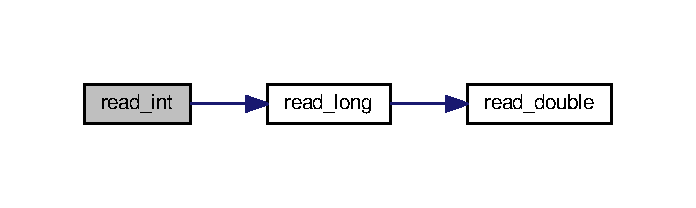
\includegraphics[width=334pt]{console__input_8h_ad0ccfbb50d0e333ef8acfeab2b7d8071_cgraph}
\end{center}
\end{figure}


\hypertarget{console__input_8h_aaaf3786f6b4803f3120609011de4b0db}{\index{console\-\_\-input.\-h@{console\-\_\-input.\-h}!read\-\_\-int@{read\-\_\-int}}
\index{read\-\_\-int@{read\-\_\-int}!console_input.h@{console\-\_\-input.\-h}}
\subsubsection[{read\-\_\-int}]{\setlength{\rightskip}{0pt plus 5cm}int read\-\_\-int (
\begin{DoxyParamCaption}
\item[{string}]{text}
\end{DoxyParamCaption}
)}}\label{console__input_8h_aaaf3786f6b4803f3120609011de4b0db}
Prints a text to the console and reads a integer value from the console in between the whole range of integer.


\begin{DoxyParams}{Parameters}
{\em text} & text to print to the console.\\
\hline
\end{DoxyParams}
\begin{DoxyReturn}{Returns}
a valid integer value. 
\end{DoxyReturn}


Here is the call graph for this function\-:\nopagebreak
\begin{figure}[H]
\begin{center}
\leavevmode
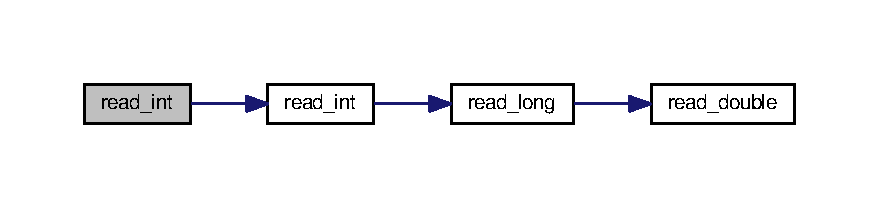
\includegraphics[width=350pt]{console__input_8h_aaaf3786f6b4803f3120609011de4b0db_cgraph}
\end{center}
\end{figure}


\hypertarget{console__input_8h_af310540093ee953c3018bc13bbde3da5}{\index{console\-\_\-input.\-h@{console\-\_\-input.\-h}!read\-\_\-int@{read\-\_\-int}}
\index{read\-\_\-int@{read\-\_\-int}!console_input.h@{console\-\_\-input.\-h}}
\subsubsection[{read\-\_\-int}]{\setlength{\rightskip}{0pt plus 5cm}int read\-\_\-int (
\begin{DoxyParamCaption}
{}
\end{DoxyParamCaption}
)}}\label{console__input_8h_af310540093ee953c3018bc13bbde3da5}
Reads an integer value from the terminal in between the whole range of long.

\begin{DoxyReturn}{Returns}
a valid integer value. 
\end{DoxyReturn}


Here is the call graph for this function\-:\nopagebreak
\begin{figure}[H]
\begin{center}
\leavevmode
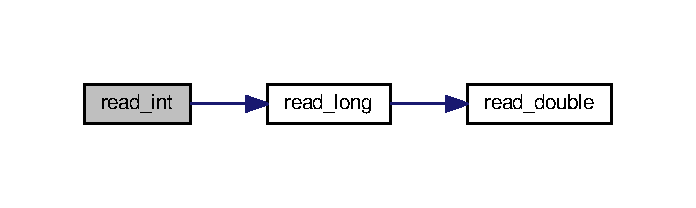
\includegraphics[width=334pt]{console__input_8h_af310540093ee953c3018bc13bbde3da5_cgraph}
\end{center}
\end{figure}


\hypertarget{console__input_8h_a03ebbd2a45117ee03be4e9002210ab36}{\index{console\-\_\-input.\-h@{console\-\_\-input.\-h}!read\-\_\-long@{read\-\_\-long}}
\index{read\-\_\-long@{read\-\_\-long}!console_input.h@{console\-\_\-input.\-h}}
\subsubsection[{read\-\_\-long}]{\setlength{\rightskip}{0pt plus 5cm}long read\-\_\-long (
\begin{DoxyParamCaption}
\item[{string}]{text, }
\item[{long}]{min, }
\item[{long}]{max}
\end{DoxyParamCaption}
)}}\label{console__input_8h_a03ebbd2a45117ee03be4e9002210ab36}
Prints a text to the console and reads a long value in between a given interval from the console. When the value is not in between the interval, the user gets prompted to reeinter a valid value.


\begin{DoxyParams}{Parameters}
{\em text} & text to print to the console. \\
\hline
{\em min} & lower bound of the interval. \\
\hline
{\em max} & top bound of the interval.\\
\hline
\end{DoxyParams}
\begin{DoxyReturn}{Returns}
a long value in between min and max. 
\end{DoxyReturn}


Here is the call graph for this function\-:\nopagebreak
\begin{figure}[H]
\begin{center}
\leavevmode
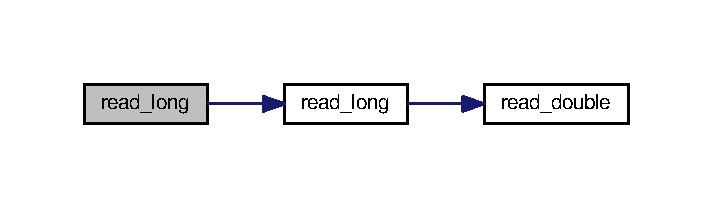
\includegraphics[width=342pt]{console__input_8h_a03ebbd2a45117ee03be4e9002210ab36_cgraph}
\end{center}
\end{figure}


\hypertarget{console__input_8h_a710a686867142de265860584f4147592}{\index{console\-\_\-input.\-h@{console\-\_\-input.\-h}!read\-\_\-long@{read\-\_\-long}}
\index{read\-\_\-long@{read\-\_\-long}!console_input.h@{console\-\_\-input.\-h}}
\subsubsection[{read\-\_\-long}]{\setlength{\rightskip}{0pt plus 5cm}long read\-\_\-long (
\begin{DoxyParamCaption}
\item[{long}]{min, }
\item[{long}]{max}
\end{DoxyParamCaption}
)}}\label{console__input_8h_a710a686867142de265860584f4147592}
Reads a long value in between a given interval from the console. When the entered value is not valid to the interval, the user gets prompted to reenter a valid.


\begin{DoxyParams}{Parameters}
{\em min} & lower bound of the interval. \\
\hline
{\em max} & top bound of the interval\\
\hline
\end{DoxyParams}
\begin{DoxyReturn}{Returns}
a long value in between min and max. 
\end{DoxyReturn}


Here is the call graph for this function\-:\nopagebreak
\begin{figure}[H]
\begin{center}
\leavevmode
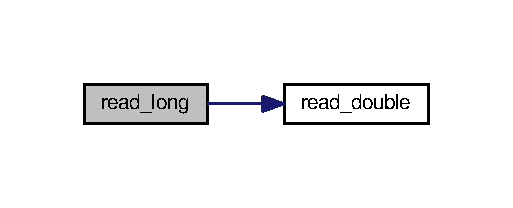
\includegraphics[width=246pt]{console__input_8h_a710a686867142de265860584f4147592_cgraph}
\end{center}
\end{figure}


\hypertarget{console__input_8h_a9128c63513d87af5259597d8c9930476}{\index{console\-\_\-input.\-h@{console\-\_\-input.\-h}!read\-\_\-long@{read\-\_\-long}}
\index{read\-\_\-long@{read\-\_\-long}!console_input.h@{console\-\_\-input.\-h}}
\subsubsection[{read\-\_\-long}]{\setlength{\rightskip}{0pt plus 5cm}long read\-\_\-long (
\begin{DoxyParamCaption}
\item[{string}]{text}
\end{DoxyParamCaption}
)}}\label{console__input_8h_a9128c63513d87af5259597d8c9930476}
Prints a text to the console and reads a long value from the console in between the whole range of long.


\begin{DoxyParams}{Parameters}
{\em text} & text to print to the console.\\
\hline
\end{DoxyParams}
\begin{DoxyReturn}{Returns}
a valid long value. 
\end{DoxyReturn}


Here is the call graph for this function\-:\nopagebreak
\begin{figure}[H]
\begin{center}
\leavevmode
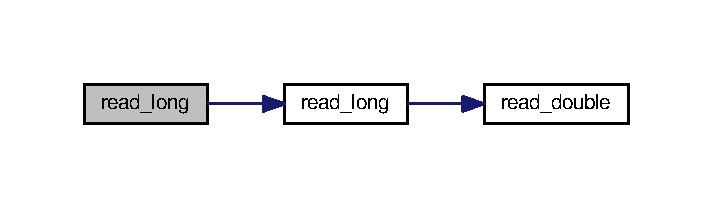
\includegraphics[width=342pt]{console__input_8h_a9128c63513d87af5259597d8c9930476_cgraph}
\end{center}
\end{figure}


\hypertarget{console__input_8h_a347c616893b725a74f60ea1f7ee325d2}{\index{console\-\_\-input.\-h@{console\-\_\-input.\-h}!read\-\_\-long@{read\-\_\-long}}
\index{read\-\_\-long@{read\-\_\-long}!console_input.h@{console\-\_\-input.\-h}}
\subsubsection[{read\-\_\-long}]{\setlength{\rightskip}{0pt plus 5cm}long read\-\_\-long (
\begin{DoxyParamCaption}
{}
\end{DoxyParamCaption}
)}}\label{console__input_8h_a347c616893b725a74f60ea1f7ee325d2}
Reads a long value from the terminal in between the whole range of long.

\begin{DoxyReturn}{Returns}
a valid long value. 
\end{DoxyReturn}


Here is the call graph for this function\-:\nopagebreak
\begin{figure}[H]
\begin{center}
\leavevmode
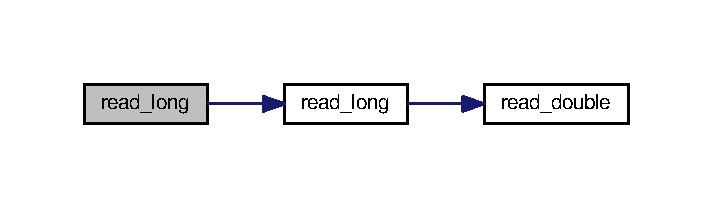
\includegraphics[width=342pt]{console__input_8h_a347c616893b725a74f60ea1f7ee325d2_cgraph}
\end{center}
\end{figure}


\hypertarget{console__input_8h_a44ccadd65be527f89bdcf6d27a3b1147}{\index{console\-\_\-input.\-h@{console\-\_\-input.\-h}!read\-\_\-text@{read\-\_\-text}}
\index{read\-\_\-text@{read\-\_\-text}!console_input.h@{console\-\_\-input.\-h}}
\subsubsection[{read\-\_\-text}]{\setlength{\rightskip}{0pt plus 5cm}string read\-\_\-text (
\begin{DoxyParamCaption}
\item[{string}]{text}
\end{DoxyParamCaption}
)}}\label{console__input_8h_a44ccadd65be527f89bdcf6d27a3b1147}
\hypertarget{console__input_8h_a6bac3909a28fff2736a171022343380b}{\index{console\-\_\-input.\-h@{console\-\_\-input.\-h}!read\-\_\-yes\-\_\-no@{read\-\_\-yes\-\_\-no}}
\index{read\-\_\-yes\-\_\-no@{read\-\_\-yes\-\_\-no}!console_input.h@{console\-\_\-input.\-h}}
\subsubsection[{read\-\_\-yes\-\_\-no}]{\setlength{\rightskip}{0pt plus 5cm}bool read\-\_\-yes\-\_\-no (
\begin{DoxyParamCaption}
\item[{string}]{text}
\end{DoxyParamCaption}
)}}\label{console__input_8h_a6bac3909a28fff2736a171022343380b}

\hypertarget{destination_8h}{\section{destination.\-h File Reference}
\label{destination_8h}\index{destination.\-h@{destination.\-h}}
}
{\ttfamily \#include $<$string$>$}\\*
Include dependency graph for destination.\-h\-:\nopagebreak
\begin{figure}[H]
\begin{center}
\leavevmode
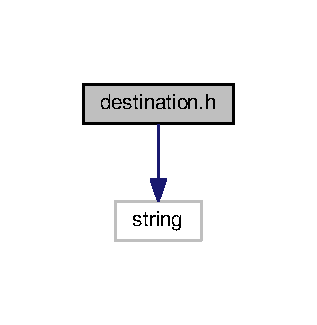
\includegraphics[width=152pt]{destination_8h__incl}
\end{center}
\end{figure}
This graph shows which files directly or indirectly include this file\-:\nopagebreak
\begin{figure}[H]
\begin{center}
\leavevmode
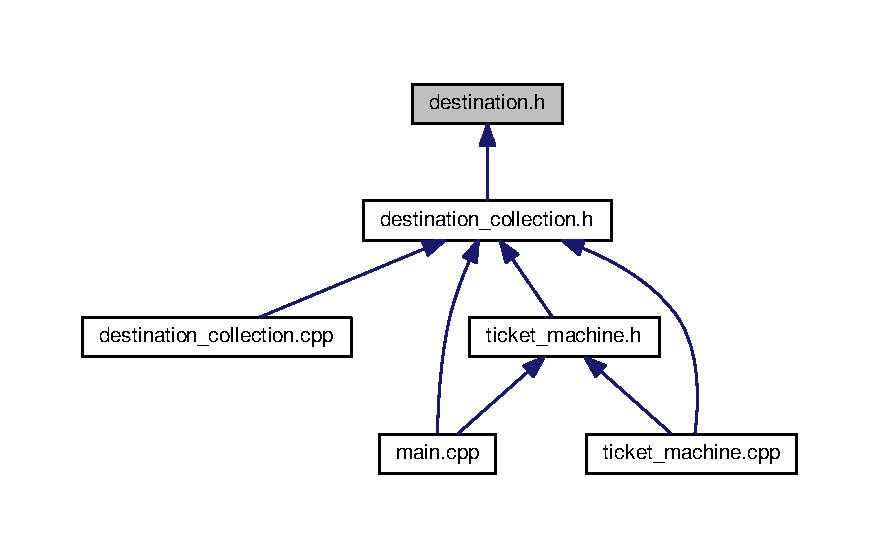
\includegraphics[width=350pt]{destination_8h__dep__incl}
\end{center}
\end{figure}
\subsection*{Classes}
\begin{DoxyCompactItemize}
\item 
struct \hyperlink{structDestination}{Destination}
\end{DoxyCompactItemize}

\hypertarget{destination__collection_8cpp}{\section{destination\-\_\-collection.\-cpp File Reference}
\label{destination__collection_8cpp}\index{destination\-\_\-collection.\-cpp@{destination\-\_\-collection.\-cpp}}
}
{\ttfamily \#include $<$iostream$>$}\\*
{\ttfamily \#include $<$iomanip$>$}\\*
{\ttfamily \#include \char`\"{}destination\-\_\-collection.\-h\char`\"{}}\\*
Include dependency graph for destination\-\_\-collection.\-cpp\-:\nopagebreak
\begin{figure}[H]
\begin{center}
\leavevmode
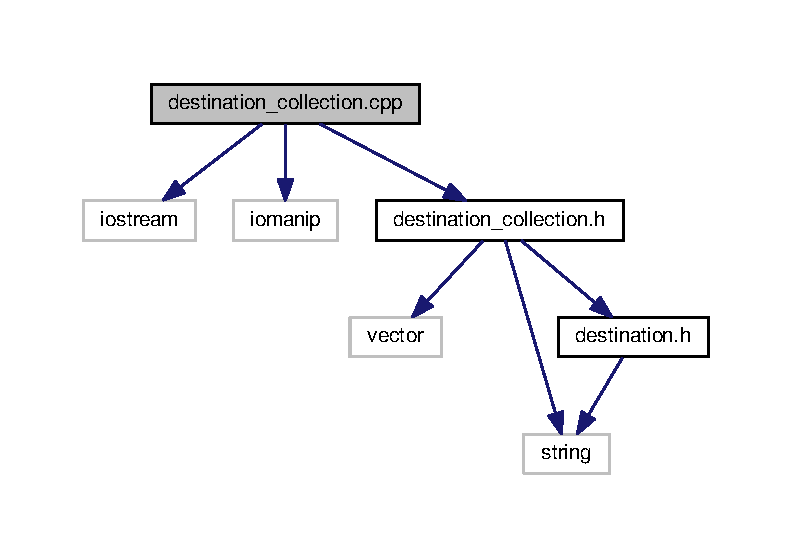
\includegraphics[width=350pt]{destination__collection_8cpp__incl}
\end{center}
\end{figure}
\subsection*{Functions}
\begin{DoxyCompactItemize}
\item 
ostream \& \hyperlink{destination__collection_8cpp_a3510520a02007ff52bce3fe80ecefa16}{operator$<$$<$} (ostream \&output, const \hyperlink{classDestinationCollection}{Destination\-Collection} \&destinations)
\end{DoxyCompactItemize}


\subsection{Function Documentation}
\hypertarget{destination__collection_8cpp_a3510520a02007ff52bce3fe80ecefa16}{\index{destination\-\_\-collection.\-cpp@{destination\-\_\-collection.\-cpp}!operator$<$$<$@{operator$<$$<$}}
\index{operator$<$$<$@{operator$<$$<$}!destination_collection.cpp@{destination\-\_\-collection.\-cpp}}
\subsubsection[{operator$<$$<$}]{\setlength{\rightskip}{0pt plus 5cm}ostream\& operator$<$$<$ (
\begin{DoxyParamCaption}
\item[{ostream \&}]{output, }
\item[{const {\bf Destination\-Collection} \&}]{destinations}
\end{DoxyParamCaption}
)}}\label{destination__collection_8cpp_a3510520a02007ff52bce3fe80ecefa16}
Overrides operator$<$$<$ \char`\"{}put to\char`\"{}. Defines how to represent a \hyperlink{classDestinationCollection}{Destination\-Collection} when print out to the console.

Vorhandene Fahrziele\-: Ziffer Fahrziel Preis \par
 1 Fahrziel 1 10.\-00 \par
 2 Fahrziel 2 5.\-00 \par
 ...\par
\par



\begin{DoxyParams}{Parameters}
{\em output} & I\-O output stream \\
\hline
{\em destinations} & The \hyperlink{classDestinationCollection}{Destination\-Collection} to print to the console.\\
\hline
\end{DoxyParams}
\begin{DoxyReturn}{Returns}
the io output stream. 
\end{DoxyReturn}


Here is the call graph for this function\-:\nopagebreak
\begin{figure}[H]
\begin{center}
\leavevmode
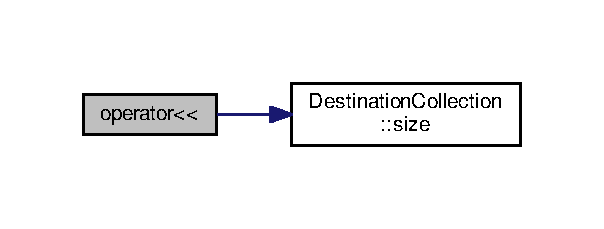
\includegraphics[width=290pt]{destination__collection_8cpp_a3510520a02007ff52bce3fe80ecefa16_cgraph}
\end{center}
\end{figure}



\hypertarget{destination__collection_8h}{\section{destination\-\_\-collection.\-h File Reference}
\label{destination__collection_8h}\index{destination\-\_\-collection.\-h@{destination\-\_\-collection.\-h}}
}
{\ttfamily \#include $<$vector$>$}\\*
{\ttfamily \#include $<$string$>$}\\*
{\ttfamily \#include \char`\"{}destination.\-h\char`\"{}}\\*
Include dependency graph for destination\-\_\-collection.\-h\-:\nopagebreak
\begin{figure}[H]
\begin{center}
\leavevmode
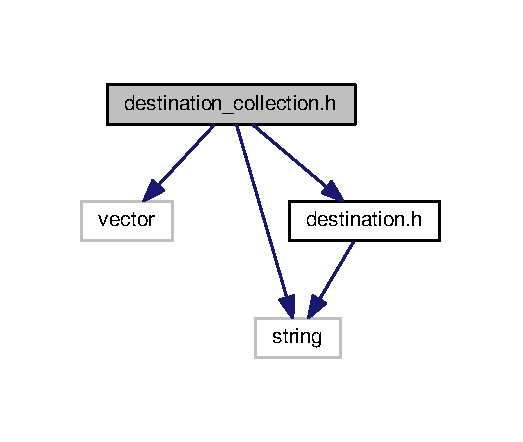
\includegraphics[width=251pt]{destination__collection_8h__incl}
\end{center}
\end{figure}
This graph shows which files directly or indirectly include this file\-:\nopagebreak
\begin{figure}[H]
\begin{center}
\leavevmode
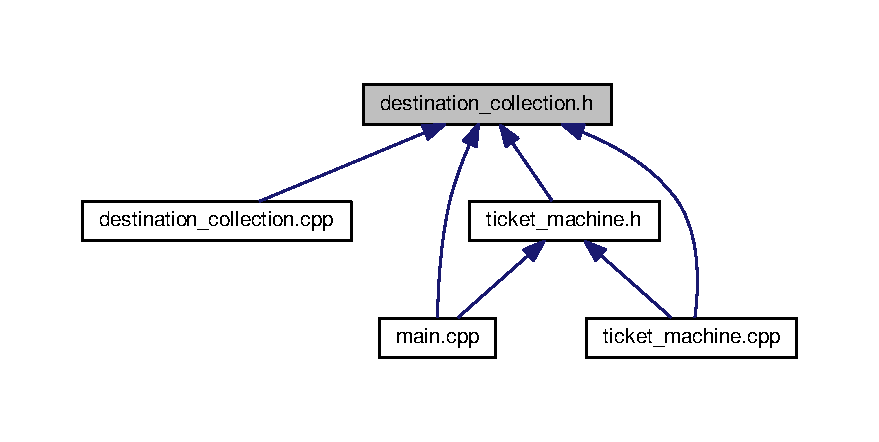
\includegraphics[width=350pt]{destination__collection_8h__dep__incl}
\end{center}
\end{figure}
\subsection*{Classes}
\begin{DoxyCompactItemize}
\item 
class \hyperlink{classDestinationCollection}{Destination\-Collection}
\end{DoxyCompactItemize}
\subsection*{Functions}
\begin{DoxyCompactItemize}
\item 
ostream \& \hyperlink{destination__collection_8h_a3510520a02007ff52bce3fe80ecefa16}{operator$<$$<$} (ostream \&output, const \hyperlink{classDestinationCollection}{Destination\-Collection} \&destinations)
\end{DoxyCompactItemize}


\subsection{Function Documentation}
\hypertarget{destination__collection_8h_a3510520a02007ff52bce3fe80ecefa16}{\index{destination\-\_\-collection.\-h@{destination\-\_\-collection.\-h}!operator$<$$<$@{operator$<$$<$}}
\index{operator$<$$<$@{operator$<$$<$}!destination_collection.h@{destination\-\_\-collection.\-h}}
\subsubsection[{operator$<$$<$}]{\setlength{\rightskip}{0pt plus 5cm}ostream\& operator$<$$<$ (
\begin{DoxyParamCaption}
\item[{ostream \&}]{output, }
\item[{const {\bf Destination\-Collection} \&}]{destinations}
\end{DoxyParamCaption}
)}}\label{destination__collection_8h_a3510520a02007ff52bce3fe80ecefa16}
Overrides operator$<$$<$ \char`\"{}put to\char`\"{}. Defines how to represent a \hyperlink{classDestinationCollection}{Destination\-Collection} when print out to the console.

Vorhandene Fahrziele\-: Ziffer Fahrziel Preis \par
 1 Fahrziel 1 10.\-00 \par
 2 Fahrziel 2 5.\-00 \par
 ...\par
\par



\begin{DoxyParams}{Parameters}
{\em output} & I\-O output stream \\
\hline
{\em destinations} & The \hyperlink{classDestinationCollection}{Destination\-Collection} to print to the console.\\
\hline
\end{DoxyParams}
\begin{DoxyReturn}{Returns}
the io output stream. 
\end{DoxyReturn}


Here is the call graph for this function\-:\nopagebreak
\begin{figure}[H]
\begin{center}
\leavevmode
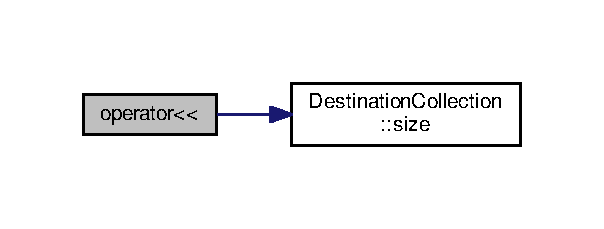
\includegraphics[width=290pt]{destination__collection_8h_a3510520a02007ff52bce3fe80ecefa16_cgraph}
\end{center}
\end{figure}



\hypertarget{main_8cpp}{\section{main.\-cpp File Reference}
\label{main_8cpp}\index{main.\-cpp@{main.\-cpp}}
}
{\ttfamily \#include $<$iostream$>$}\\*
{\ttfamily \#include $<$iomanip$>$}\\*
{\ttfamily \#include $<$string$>$}\\*
{\ttfamily \#include \char`\"{}maumau.\-h\char`\"{}}\\*
Include dependency graph for main.\-cpp\-:\nopagebreak
\begin{figure}[H]
\begin{center}
\leavevmode
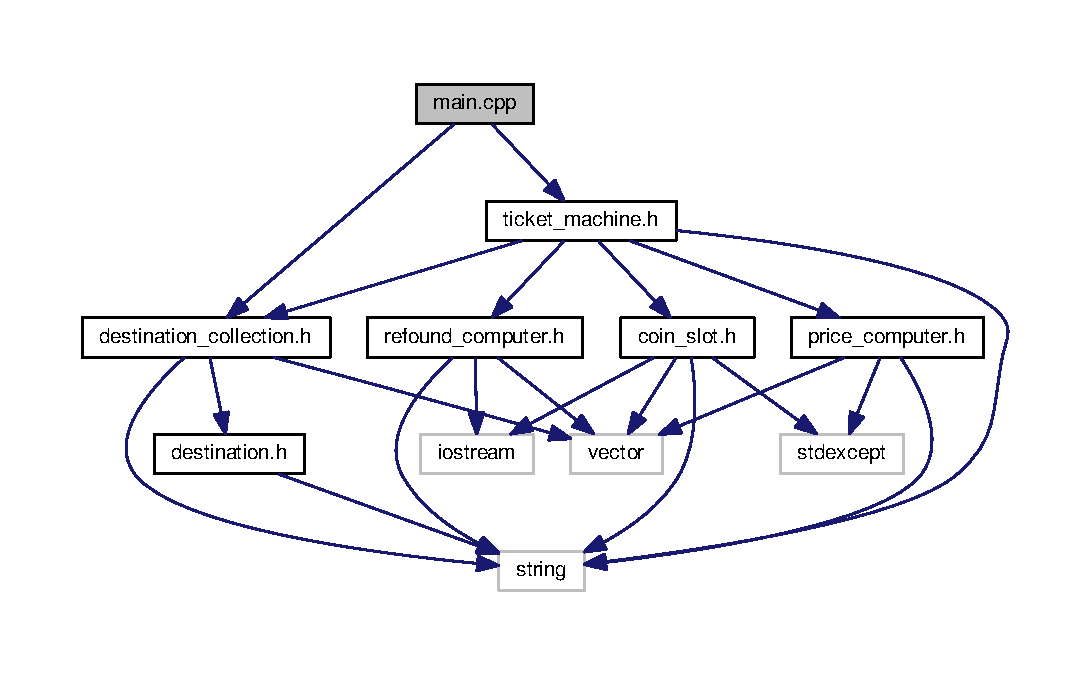
\includegraphics[width=350pt]{main_8cpp__incl}
\end{center}
\end{figure}
\subsection*{Functions}
\begin{DoxyCompactItemize}
\item 
void \hyperlink{main_8cpp_ad45e149aada26b44cb0274a5eb865edb}{print\-\_\-manual} ()
\item 
int \hyperlink{main_8cpp_a0ddf1224851353fc92bfbff6f499fa97}{main} (int argc, char $\ast$argv\mbox{[}$\,$\mbox{]})
\end{DoxyCompactItemize}


\subsection{Function Documentation}
\hypertarget{main_8cpp_a0ddf1224851353fc92bfbff6f499fa97}{\index{main.\-cpp@{main.\-cpp}!main@{main}}
\index{main@{main}!main.cpp@{main.\-cpp}}
\subsubsection[{main}]{\setlength{\rightskip}{0pt plus 5cm}int main (
\begin{DoxyParamCaption}
\item[{int}]{argc, }
\item[{char $\ast$}]{argv\mbox{[}$\,$\mbox{]}}
\end{DoxyParamCaption}
)}}\label{main_8cpp_a0ddf1224851353fc92bfbff6f499fa97}
Entrypoint to the program \char`\"{}\-Maumau\char`\"{}. Checks the arguments given by the user and starts a new game for four players. When the option -\/a is set the game gets completely simulated. When the option -\/m is set the User will play the \hyperlink{classPlayer}{Player} 1. If the program gets started with invalid parameters, there is a manual shown. 

Here is the call graph for this function\-:\nopagebreak
\begin{figure}[H]
\begin{center}
\leavevmode
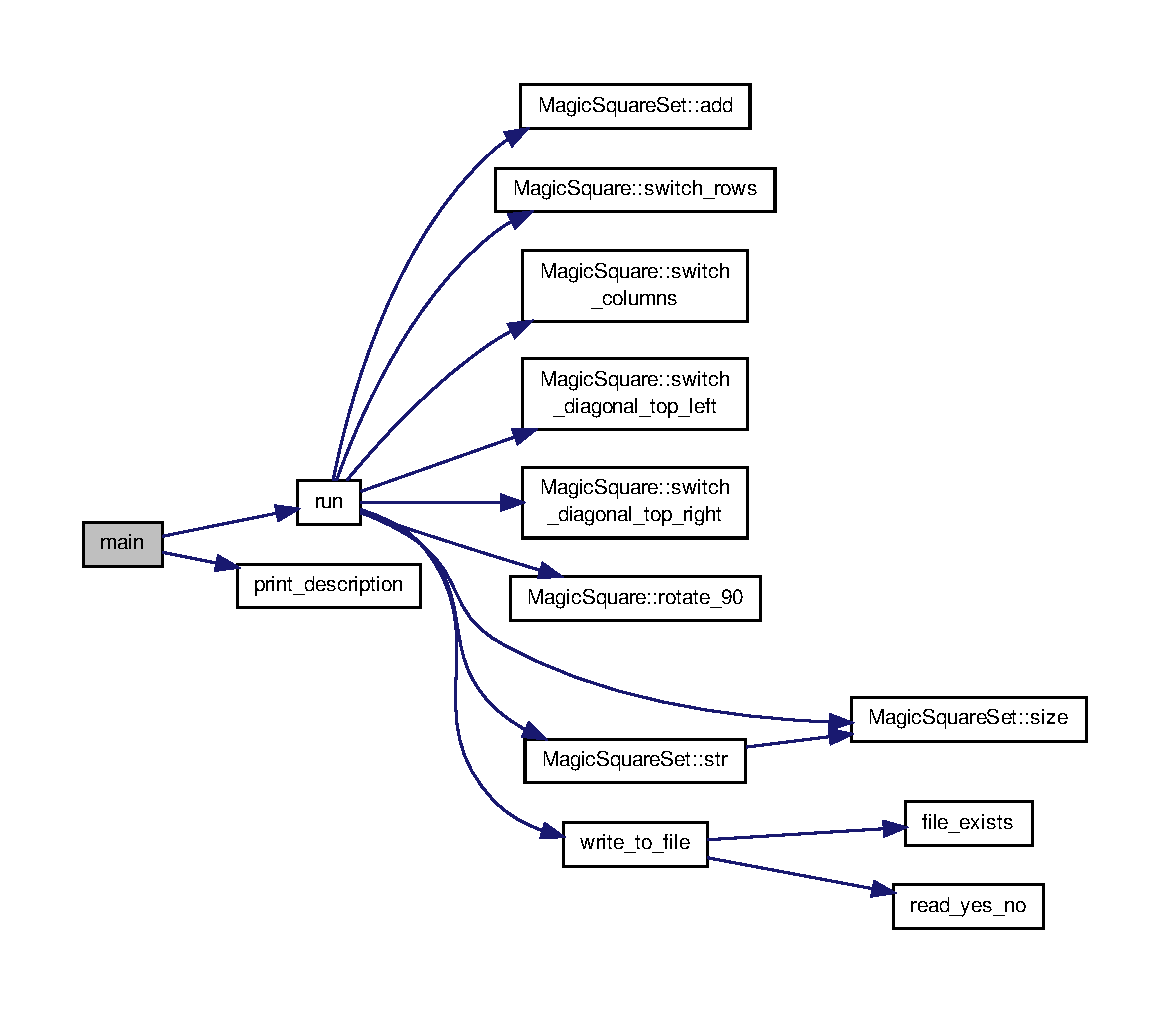
\includegraphics[width=350pt]{main_8cpp_a0ddf1224851353fc92bfbff6f499fa97_cgraph}
\end{center}
\end{figure}


\hypertarget{main_8cpp_ad45e149aada26b44cb0274a5eb865edb}{\index{main.\-cpp@{main.\-cpp}!print\-\_\-manual@{print\-\_\-manual}}
\index{print\-\_\-manual@{print\-\_\-manual}!main.cpp@{main.\-cpp}}
\subsubsection[{print\-\_\-manual}]{\setlength{\rightskip}{0pt plus 5cm}void print\-\_\-manual (
\begin{DoxyParamCaption}
{}
\end{DoxyParamCaption}
)}}\label{main_8cpp_ad45e149aada26b44cb0274a5eb865edb}

\hypertarget{main_8h}{\section{main.\-h File Reference}
\label{main_8h}\index{main.\-h@{main.\-h}}
}
{\ttfamily \#include \char`\"{}fraction.\-h\char`\"{}}\\*
{\ttfamily \#include $<$string$>$}\\*
{\ttfamily \#include $<$vector$>$}\\*
Include dependency graph for main.\-h\-:\nopagebreak
\begin{figure}[H]
\begin{center}
\leavevmode
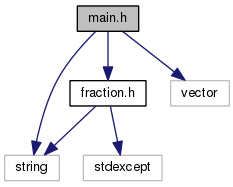
\includegraphics[width=247pt]{main_8h__incl}
\end{center}
\end{figure}
This graph shows which files directly or indirectly include this file\-:\nopagebreak
\begin{figure}[H]
\begin{center}
\leavevmode
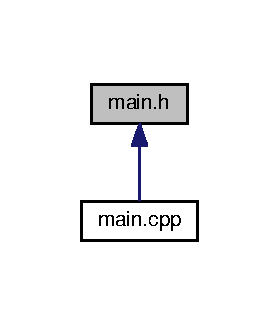
\includegraphics[width=134pt]{main_8h__dep__incl}
\end{center}
\end{figure}
\subsection*{Typedefs}
\begin{DoxyCompactItemize}
\item 
typedef \hyperlink{classFraction}{Fraction}(Fraction\-::$\ast$ \hyperlink{main_8h_a9b6408a5e81c4f9a51ed827e8c7ca6b3}{fptr} )(const \hyperlink{classFraction}{Fraction} \&) const 
\item 
typedef \hyperlink{classFraction}{Fraction}(Fraction\-::$\ast$ \hyperlink{main_8h_a418b3bd910bac84dd93361a1c0400690}{fptr2} )(const int \&) const 
\item 
typedef \hyperlink{classFraction}{Fraction}($\ast$ \hyperlink{main_8h_aa046d174f627935ab5810e02c246e7b3}{fptr3} )(const int \&, const \hyperlink{classFraction}{Fraction} \&)
\end{DoxyCompactItemize}
\subsection*{Functions}
\begin{DoxyCompactItemize}
\item 
void \hyperlink{main_8h_a88a5a1f559a0f664dbb99b66f6c86c59}{handle\-\_\-five} (char $\ast$argv\mbox{[}$\,$\mbox{]})
\item 
void \hyperlink{main_8h_afbc888f515c7c31845c525098c70a949}{handle\-\_\-six} (char $\ast$argv\mbox{[}$\,$\mbox{]})
\item 
void \hyperlink{main_8h_a6d598685a1aa70dc69dc3d66f694415d}{handle\-\_\-nine} (char $\ast$argv\mbox{[}$\,$\mbox{]})
\item 
void \hyperlink{main_8h_a24574ed2cace07e9d96f9cf8c14e9fa6}{sort} (std\-::vector$<$ \hyperlink{classFraction}{Fraction} $>$ \&array, int length, bool asc)
\item 
std\-::vector$<$ \hyperlink{classFraction}{Fraction} $>$ \hyperlink{main_8h_a7bc0d7d99bb9ae80f7ab54fcd1d3da01}{random\-\_\-fractions} (int amounth, int low\-\_\-numerator, int low\-\_\-denominator, int high\-\_\-numerator, int high\-\_\-denominator)  throw (const std\-::invalid\-\_\-argument)
\item 
void \hyperlink{main_8h_a45ba46a5ae34b55a833eced785f695ea}{random\-\_\-handler} (int n, int a, int b, int c, int d, bool asc)
\item 
bool \hyperlink{main_8h_a1920cd03342937f72cb6c49041a6953d}{isi} (char text\mbox{[}$\,$\mbox{]})
\item 
void \hyperlink{main_8h_a7c827c26e5661b0c05da029a209d0cb8}{show\-\_\-manual} ()
\end{DoxyCompactItemize}


\subsection{Typedef Documentation}
\hypertarget{main_8h_a9b6408a5e81c4f9a51ed827e8c7ca6b3}{\index{main.\-h@{main.\-h}!fptr@{fptr}}
\index{fptr@{fptr}!main.h@{main.\-h}}
\subsubsection[{fptr}]{\setlength{\rightskip}{0pt plus 5cm}typedef {\bf Fraction}(Fraction\-::$\ast$ fptr)(const {\bf Fraction} \&) const }}\label{main_8h_a9b6408a5e81c4f9a51ed827e8c7ca6b3}
\hypertarget{main_8h_a418b3bd910bac84dd93361a1c0400690}{\index{main.\-h@{main.\-h}!fptr2@{fptr2}}
\index{fptr2@{fptr2}!main.h@{main.\-h}}
\subsubsection[{fptr2}]{\setlength{\rightskip}{0pt plus 5cm}typedef {\bf Fraction}(Fraction\-::$\ast$ fptr2)(const int \&) const }}\label{main_8h_a418b3bd910bac84dd93361a1c0400690}
\hypertarget{main_8h_aa046d174f627935ab5810e02c246e7b3}{\index{main.\-h@{main.\-h}!fptr3@{fptr3}}
\index{fptr3@{fptr3}!main.h@{main.\-h}}
\subsubsection[{fptr3}]{\setlength{\rightskip}{0pt plus 5cm}typedef {\bf Fraction}($\ast$ fptr3)(const int \&, const {\bf Fraction} \&)}}\label{main_8h_aa046d174f627935ab5810e02c246e7b3}


\subsection{Function Documentation}
\hypertarget{main_8h_a88a5a1f559a0f664dbb99b66f6c86c59}{\index{main.\-h@{main.\-h}!handle\-\_\-five@{handle\-\_\-five}}
\index{handle\-\_\-five@{handle\-\_\-five}!main.h@{main.\-h}}
\subsubsection[{handle\-\_\-five}]{\setlength{\rightskip}{0pt plus 5cm}void handle\-\_\-five (
\begin{DoxyParamCaption}
\item[{char $\ast$}]{argv\mbox{[}$\,$\mbox{]}}
\end{DoxyParamCaption}
)}}\label{main_8h_a88a5a1f559a0f664dbb99b66f6c86c59}
Handles program when executed with five arguments. Validates input format.

Possible actions are\-: bruch a op c d a op c/d = e/f =$>$ bruch 1 -\/ 1 2 1 -\/ 1/2 = 1/2 bruch a b op c a/b op c = e/f =$>$ bruch 1 2 -\/ 1 1/2 -\/ 1 = -\/1/2


\begin{DoxyParams}{Parameters}
{\em $\ast$argv\mbox{[}$\,$\mbox{]}} & Arguments array form the program execution. \\
\hline
\end{DoxyParams}


Here is the call graph for this function\-:\nopagebreak
\begin{figure}[H]
\begin{center}
\leavevmode
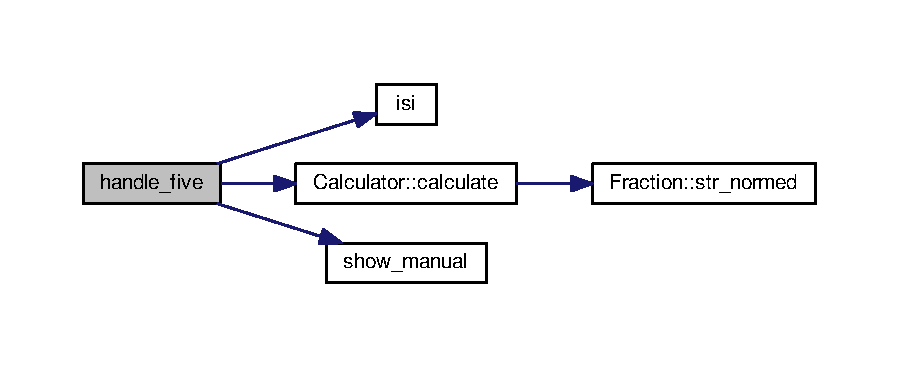
\includegraphics[width=350pt]{main_8h_a88a5a1f559a0f664dbb99b66f6c86c59_cgraph}
\end{center}
\end{figure}


\hypertarget{main_8h_a6d598685a1aa70dc69dc3d66f694415d}{\index{main.\-h@{main.\-h}!handle\-\_\-nine@{handle\-\_\-nine}}
\index{handle\-\_\-nine@{handle\-\_\-nine}!main.h@{main.\-h}}
\subsubsection[{handle\-\_\-nine}]{\setlength{\rightskip}{0pt plus 5cm}void handle\-\_\-nine (
\begin{DoxyParamCaption}
\item[{char $\ast$}]{argv\mbox{[}$\,$\mbox{]}}
\end{DoxyParamCaption}
)}}\label{main_8h_a6d598685a1aa70dc69dc3d66f694415d}
Handles program when executed with nine arguments. Validates input format.

Possible actions are\-: bruch n \mbox{[} a b c d \mbox{]} + n numbers between a/b and c/d ascendent sorted. bruch n \mbox{[} a b c d \mbox{]} -\/ n numbers between a/b and c/d descendent sorted.


\begin{DoxyParams}{Parameters}
{\em $\ast$argv\mbox{[}$\,$\mbox{]}} & Arguments array form the program execution. \\
\hline
\end{DoxyParams}


Here is the call graph for this function\-:\nopagebreak
\begin{figure}[H]
\begin{center}
\leavevmode
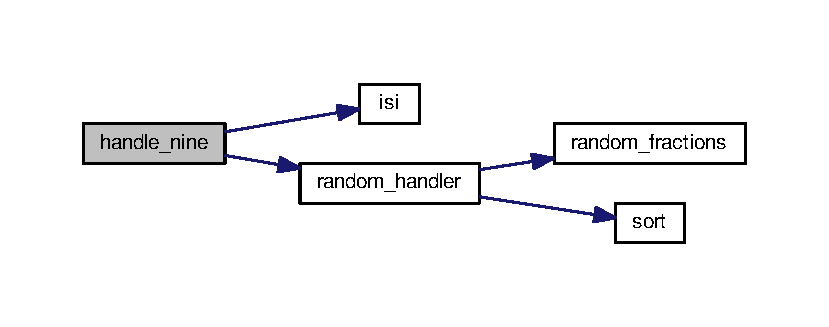
\includegraphics[width=350pt]{main_8h_a6d598685a1aa70dc69dc3d66f694415d_cgraph}
\end{center}
\end{figure}


\hypertarget{main_8h_afbc888f515c7c31845c525098c70a949}{\index{main.\-h@{main.\-h}!handle\-\_\-six@{handle\-\_\-six}}
\index{handle\-\_\-six@{handle\-\_\-six}!main.h@{main.\-h}}
\subsubsection[{handle\-\_\-six}]{\setlength{\rightskip}{0pt plus 5cm}void handle\-\_\-six (
\begin{DoxyParamCaption}
\item[{char $\ast$}]{argv\mbox{[}$\,$\mbox{]}}
\end{DoxyParamCaption}
)}}\label{main_8h_afbc888f515c7c31845c525098c70a949}
Handles program when executed with six arguments. Validates input format.

Possible actions are\-: bruch a b op c d a/b op c/d = e/f =$>$ bruch 1 2 -\/ 1 3 1/2 -\/ 1/3 = 1/6 bruch a b -\/v c d a/b \mbox{[}$<$$\vert$$>$$\vert$=\mbox{]} c/d =$>$ 1 2 -\/v 1 3 1/2 $>$ 1/3


\begin{DoxyParams}{Parameters}
{\em $\ast$argv\mbox{[}$\,$\mbox{]}} & Arguments array form the program execution. \\
\hline
\end{DoxyParams}


Here is the call graph for this function\-:\nopagebreak
\begin{figure}[H]
\begin{center}
\leavevmode
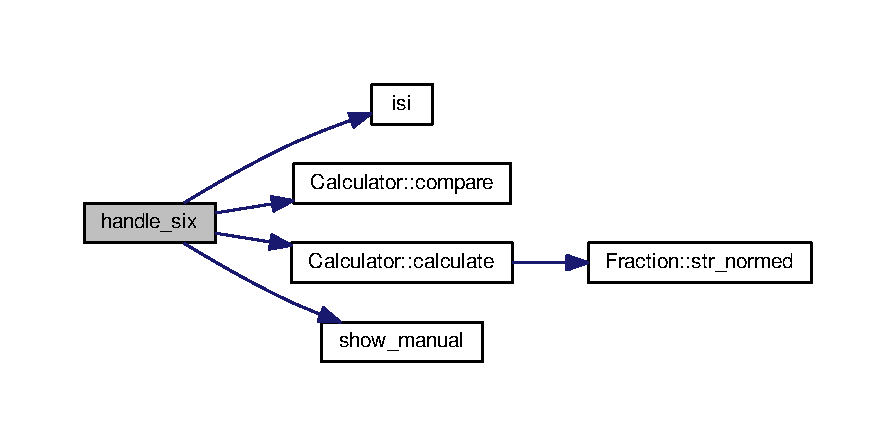
\includegraphics[width=350pt]{main_8h_afbc888f515c7c31845c525098c70a949_cgraph}
\end{center}
\end{figure}


\hypertarget{main_8h_a1920cd03342937f72cb6c49041a6953d}{\index{main.\-h@{main.\-h}!isi@{isi}}
\index{isi@{isi}!main.h@{main.\-h}}
\subsubsection[{isi}]{\setlength{\rightskip}{0pt plus 5cm}bool isi (
\begin{DoxyParamCaption}
\item[{char}]{text\mbox{[}$\,$\mbox{]}}
\end{DoxyParamCaption}
)}}\label{main_8h_a1920cd03342937f72cb6c49041a6953d}
Checks whether an array of chars represents an integer or not. Solfs atoi problem that returns a 0 for a char which is not a number.


\begin{DoxyParams}{Parameters}
{\em text\mbox{[}$\,$\mbox{]}} & Array of chars.\\
\hline
\end{DoxyParams}
\begin{DoxyReturn}{Returns}
true when text\mbox{[}\mbox{]} represents a number. false when text\mbox{[}\mbox{]} doesn't represent a number. 
\end{DoxyReturn}
\hypertarget{main_8h_a7bc0d7d99bb9ae80f7ab54fcd1d3da01}{\index{main.\-h@{main.\-h}!random\-\_\-fractions@{random\-\_\-fractions}}
\index{random\-\_\-fractions@{random\-\_\-fractions}!main.h@{main.\-h}}
\subsubsection[{random\-\_\-fractions}]{\setlength{\rightskip}{0pt plus 5cm}std\-::vector$<${\bf Fraction}$>$ random\-\_\-fractions (
\begin{DoxyParamCaption}
\item[{int}]{n, }
\item[{int}]{low\-\_\-numerator, }
\item[{int}]{low\-\_\-denominator, }
\item[{int}]{high\-\_\-numerator, }
\item[{int}]{high\-\_\-denominator}
\end{DoxyParamCaption}
) throw  const std\-::invalid\-\_\-argument) }}\label{main_8h_a7bc0d7d99bb9ae80f7ab54fcd1d3da01}
Generates n random Fractions with value in between the Fractions a/b and c/d and gives them back as vector.


\begin{DoxyParams}{Parameters}
{\em n} & Number of random fractions. \\
\hline
{\em low\-\_\-numerator} & Numerator of the low bound fraction. \\
\hline
{\em low\-\_\-denominator} & Denominator of the low bound fraction. \\
\hline
{\em high\-\_\-numerator} & Numerator of the high bound fraction. \\
\hline
{\em high\-\_\-deominator} & Denominator of the high bound fraction.\\
\hline
\end{DoxyParams}
\begin{DoxyReturn}{Returns}
vector with the fractions. 
\end{DoxyReturn}
\hypertarget{main_8h_a45ba46a5ae34b55a833eced785f695ea}{\index{main.\-h@{main.\-h}!random\-\_\-handler@{random\-\_\-handler}}
\index{random\-\_\-handler@{random\-\_\-handler}!main.h@{main.\-h}}
\subsubsection[{random\-\_\-handler}]{\setlength{\rightskip}{0pt plus 5cm}void random\-\_\-handler (
\begin{DoxyParamCaption}
\item[{int}]{n, }
\item[{int}]{a, }
\item[{int}]{b, }
\item[{int}]{c, }
\item[{int}]{d, }
\item[{bool}]{asc}
\end{DoxyParamCaption}
)}}\label{main_8h_a45ba46a5ae34b55a833eced785f695ea}
Generates n random Fractions in between the Fractions a/b and c/d, sorts them eigther ascendent or descendent according the parameter asc and prints the sorted and unsorted result to the console.


\begin{DoxyParams}{Parameters}
{\em n} & Number of random fractions. \\
\hline
{\em a} & Numerator of the low bound fraction. \\
\hline
{\em b} & Denominator of the low bound fraction. \\
\hline
{\em c} & Numerator of the high bound fraction. \\
\hline
{\em d} & Denominator of the high bound fraction. \\
\hline
{\em asc} & Deriction to sort, true =$>$ asc, false =$>$ desc. \\
\hline
\end{DoxyParams}


Here is the call graph for this function\-:\nopagebreak
\begin{figure}[H]
\begin{center}
\leavevmode
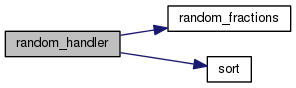
\includegraphics[width=294pt]{main_8h_a45ba46a5ae34b55a833eced785f695ea_cgraph}
\end{center}
\end{figure}


\hypertarget{main_8h_a7c827c26e5661b0c05da029a209d0cb8}{\index{main.\-h@{main.\-h}!show\-\_\-manual@{show\-\_\-manual}}
\index{show\-\_\-manual@{show\-\_\-manual}!main.h@{main.\-h}}
\subsubsection[{show\-\_\-manual}]{\setlength{\rightskip}{0pt plus 5cm}void show\-\_\-manual (
\begin{DoxyParamCaption}
{}
\end{DoxyParamCaption}
)}}\label{main_8h_a7c827c26e5661b0c05da029a209d0cb8}
Reads a file according a given filename and prints the content to the console.


\begin{DoxyParams}{Parameters}
{\em filename} & Name of the file to print to the console. \\
\hline
\end{DoxyParams}
\hypertarget{main_8h_a24574ed2cace07e9d96f9cf8c14e9fa6}{\index{main.\-h@{main.\-h}!sort@{sort}}
\index{sort@{sort}!main.h@{main.\-h}}
\subsubsection[{sort}]{\setlength{\rightskip}{0pt plus 5cm}void sort (
\begin{DoxyParamCaption}
\item[{std\-::vector$<$ {\bf Fraction} $>$ \&}]{fractions, }
\item[{int}]{length, }
\item[{bool}]{asc}
\end{DoxyParamCaption}
)}}\label{main_8h_a24574ed2cace07e9d96f9cf8c14e9fa6}
Sorts an vector of fractions with the entry sort algorithm in according to the param asc ascendent or descendent.


\begin{DoxyParams}{Parameters}
{\em fractions} & Vector with the fraction to sort. \\
\hline
{\em length} & Length of the vector. \\
\hline
{\em asc} & Direction to sort. true =$>$ asc, false =$>$ desc. \\
\hline
\end{DoxyParams}

\hypertarget{price__computer_8cpp}{\section{price\-\_\-computer.\-cpp File Reference}
\label{price__computer_8cpp}\index{price\-\_\-computer.\-cpp@{price\-\_\-computer.\-cpp}}
}
{\ttfamily \#include $<$cmath$>$}\\*
{\ttfamily \#include $<$string$>$}\\*
{\ttfamily \#include $<$sstream$>$}\\*
{\ttfamily \#include $<$iomanip$>$}\\*
{\ttfamily \#include $<$vector$>$}\\*
{\ttfamily \#include $<$stdexcept$>$}\\*
{\ttfamily \#include \char`\"{}price\-\_\-computer.\-h\char`\"{}}\\*
{\ttfamily \#include \char`\"{}refound\-\_\-computer.\-h\char`\"{}}\\*
Include dependency graph for price\-\_\-computer.\-cpp\-:\nopagebreak
\begin{figure}[H]
\begin{center}
\leavevmode
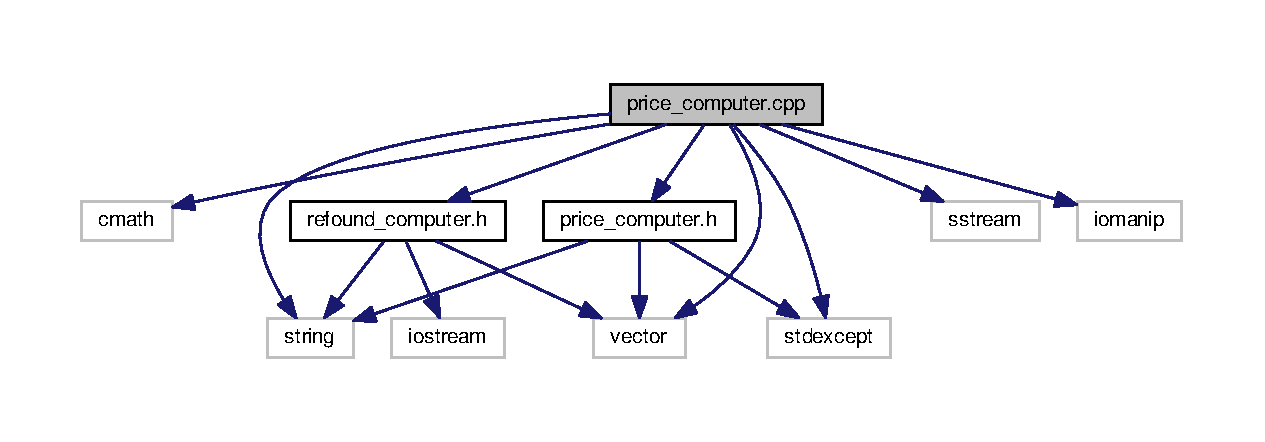
\includegraphics[width=350pt]{price__computer_8cpp__incl}
\end{center}
\end{figure}
\subsection*{Functions}
\begin{DoxyCompactItemize}
\item 
ostream \& \hyperlink{price__computer_8cpp_ad04ee4353df3d82d9f8f43db1d12575d}{operator$<$$<$} (ostream \&output, const \hyperlink{classPriceComputer}{Price\-Computer} \&pc)
\end{DoxyCompactItemize}


\subsection{Function Documentation}
\hypertarget{price__computer_8cpp_ad04ee4353df3d82d9f8f43db1d12575d}{\index{price\-\_\-computer.\-cpp@{price\-\_\-computer.\-cpp}!operator$<$$<$@{operator$<$$<$}}
\index{operator$<$$<$@{operator$<$$<$}!price_computer.cpp@{price\-\_\-computer.\-cpp}}
\subsubsection[{operator$<$$<$}]{\setlength{\rightskip}{0pt plus 5cm}ostream\& operator$<$$<$ (
\begin{DoxyParamCaption}
\item[{ostream \&}]{output, }
\item[{const {\bf Price\-Computer} \&}]{pc}
\end{DoxyParamCaption}
)}}\label{price__computer_8cpp_ad04ee4353df3d82d9f8f43db1d12575d}
Overrides the global operator$<$$<$ \char`\"{}put to\char`\"{}. Represents a \hyperlink{classPriceComputer}{Price\-Computer} when put to an output stream.


\begin{DoxyParams}{Parameters}
{\em output} & io output stream. \\
\hline
{\em pc} & \hyperlink{classPriceComputer}{Price\-Computer} to put to the output stream.\\
\hline
\end{DoxyParams}
\begin{DoxyReturn}{Returns}
the io output stream. 
\end{DoxyReturn}


Here is the call graph for this function\-:\nopagebreak
\begin{figure}[H]
\begin{center}
\leavevmode
\includegraphics[width=350pt]{price__computer_8cpp_ad04ee4353df3d82d9f8f43db1d12575d_cgraph}
\end{center}
\end{figure}



\hypertarget{price__computer_8h}{\section{price\-\_\-computer.\-h File Reference}
\label{price__computer_8h}\index{price\-\_\-computer.\-h@{price\-\_\-computer.\-h}}
}
{\ttfamily \#include $<$vector$>$}\\*
{\ttfamily \#include $<$string$>$}\\*
{\ttfamily \#include $<$stdexcept$>$}\\*
Include dependency graph for price\-\_\-computer.\-h\-:\nopagebreak
\begin{figure}[H]
\begin{center}
\leavevmode
\includegraphics[width=259pt]{price__computer_8h__incl}
\end{center}
\end{figure}
This graph shows which files directly or indirectly include this file\-:\nopagebreak
\begin{figure}[H]
\begin{center}
\leavevmode
\includegraphics[width=333pt]{price__computer_8h__dep__incl}
\end{center}
\end{figure}
\subsection*{Classes}
\begin{DoxyCompactItemize}
\item 
class \hyperlink{classPriceComputer}{Price\-Computer}
\end{DoxyCompactItemize}
\subsection*{Functions}
\begin{DoxyCompactItemize}
\item 
ostream \& \hyperlink{price__computer_8h_ad04ee4353df3d82d9f8f43db1d12575d}{operator$<$$<$} (ostream \&output, const \hyperlink{classPriceComputer}{Price\-Computer} \&pc)
\end{DoxyCompactItemize}


\subsection{Function Documentation}
\hypertarget{price__computer_8h_ad04ee4353df3d82d9f8f43db1d12575d}{\index{price\-\_\-computer.\-h@{price\-\_\-computer.\-h}!operator$<$$<$@{operator$<$$<$}}
\index{operator$<$$<$@{operator$<$$<$}!price_computer.h@{price\-\_\-computer.\-h}}
\subsubsection[{operator$<$$<$}]{\setlength{\rightskip}{0pt plus 5cm}ostream\& operator$<$$<$ (
\begin{DoxyParamCaption}
\item[{ostream \&}]{output, }
\item[{const {\bf Price\-Computer} \&}]{pc}
\end{DoxyParamCaption}
)}}\label{price__computer_8h_ad04ee4353df3d82d9f8f43db1d12575d}
Overrides the global operator$<$$<$ \char`\"{}put to\char`\"{}. Represents a \hyperlink{classPriceComputer}{Price\-Computer} when put to an output stream.


\begin{DoxyParams}{Parameters}
{\em output} & io output stream. \\
\hline
{\em pc} & \hyperlink{classPriceComputer}{Price\-Computer} to put to the output stream.\\
\hline
\end{DoxyParams}
\begin{DoxyReturn}{Returns}
the io output stream. 
\end{DoxyReturn}


Here is the call graph for this function\-:\nopagebreak
\begin{figure}[H]
\begin{center}
\leavevmode
\includegraphics[width=350pt]{price__computer_8h_ad04ee4353df3d82d9f8f43db1d12575d_cgraph}
\end{center}
\end{figure}



\hypertarget{refound__computer_8cpp}{\section{refound\-\_\-computer.\-cpp File Reference}
\label{refound__computer_8cpp}\index{refound\-\_\-computer.\-cpp@{refound\-\_\-computer.\-cpp}}
}
{\ttfamily \#include $<$iostream$>$}\\*
{\ttfamily \#include $<$sstream$>$}\\*
{\ttfamily \#include $<$iomanip$>$}\\*
{\ttfamily \#include $<$string$>$}\\*
{\ttfamily \#include \char`\"{}refound\-\_\-computer.\-h\char`\"{}}\\*
Include dependency graph for refound\-\_\-computer.\-cpp\-:\nopagebreak
\begin{figure}[H]
\begin{center}
\leavevmode
\includegraphics[width=350pt]{refound__computer_8cpp__incl}
\end{center}
\end{figure}
\subsection*{Functions}
\begin{DoxyCompactItemize}
\item 
ostream \& \hyperlink{refound__computer_8cpp_a41cc2b5a50bd1435bcdb44db3933c955}{operator$<$$<$} (ostream \&output, const \hyperlink{classRefoundComputer}{Refound\-Computer} \&refound)
\end{DoxyCompactItemize}


\subsection{Function Documentation}
\hypertarget{refound__computer_8cpp_a41cc2b5a50bd1435bcdb44db3933c955}{\index{refound\-\_\-computer.\-cpp@{refound\-\_\-computer.\-cpp}!operator$<$$<$@{operator$<$$<$}}
\index{operator$<$$<$@{operator$<$$<$}!refound_computer.cpp@{refound\-\_\-computer.\-cpp}}
\subsubsection[{operator$<$$<$}]{\setlength{\rightskip}{0pt plus 5cm}ostream\& operator$<$$<$ (
\begin{DoxyParamCaption}
\item[{ostream \&}]{output, }
\item[{const {\bf Refound\-Computer} \&}]{refound}
\end{DoxyParamCaption}
)}}\label{refound__computer_8cpp_a41cc2b5a50bd1435bcdb44db3933c955}
Overrides the global operatro$<$$<$ \char`\"{}put to\char`\"{}, for the default string representation of a Recound\-Computer in a output stream. Uses the representation defined with \hyperlink{classPriceComputer_ac6a85d7316a174de19a4eccdffd91ae3}{Price\-Computer\-::str()}.


\begin{DoxyParams}{Parameters}
{\em output} & io output stream. \\
\hline
{\em refound} & Refounc\-Computer to put to the output stream.\\
\hline
\end{DoxyParams}
\begin{DoxyReturn}{Returns}
io output stream. 
\end{DoxyReturn}


Here is the call graph for this function\-:\nopagebreak
\begin{figure}[H]
\begin{center}
\leavevmode
\includegraphics[width=294pt]{refound__computer_8cpp_a41cc2b5a50bd1435bcdb44db3933c955_cgraph}
\end{center}
\end{figure}



\hypertarget{refound__computer_8h}{\section{refound\-\_\-computer.\-h File Reference}
\label{refound__computer_8h}\index{refound\-\_\-computer.\-h@{refound\-\_\-computer.\-h}}
}
{\ttfamily \#include $<$iostream$>$}\\*
{\ttfamily \#include $<$string$>$}\\*
{\ttfamily \#include $<$vector$>$}\\*
Include dependency graph for refound\-\_\-computer.\-h\-:\nopagebreak
\begin{figure}[H]
\begin{center}
\leavevmode
\includegraphics[width=255pt]{refound__computer_8h__incl}
\end{center}
\end{figure}
This graph shows which files directly or indirectly include this file\-:\nopagebreak
\begin{figure}[H]
\begin{center}
\leavevmode
\includegraphics[width=350pt]{refound__computer_8h__dep__incl}
\end{center}
\end{figure}
\subsection*{Classes}
\begin{DoxyCompactItemize}
\item 
class \hyperlink{classRefoundComputer}{Refound\-Computer}
\end{DoxyCompactItemize}
\subsection*{Functions}
\begin{DoxyCompactItemize}
\item 
ostream \& \hyperlink{refound__computer_8h_a41cc2b5a50bd1435bcdb44db3933c955}{operator$<$$<$} (ostream \&output, const \hyperlink{classRefoundComputer}{Refound\-Computer} \&refound)
\end{DoxyCompactItemize}


\subsection{Function Documentation}
\hypertarget{refound__computer_8h_a41cc2b5a50bd1435bcdb44db3933c955}{\index{refound\-\_\-computer.\-h@{refound\-\_\-computer.\-h}!operator$<$$<$@{operator$<$$<$}}
\index{operator$<$$<$@{operator$<$$<$}!refound_computer.h@{refound\-\_\-computer.\-h}}
\subsubsection[{operator$<$$<$}]{\setlength{\rightskip}{0pt plus 5cm}ostream\& operator$<$$<$ (
\begin{DoxyParamCaption}
\item[{ostream \&}]{output, }
\item[{const {\bf Refound\-Computer} \&}]{refound}
\end{DoxyParamCaption}
)}}\label{refound__computer_8h_a41cc2b5a50bd1435bcdb44db3933c955}
Overrides the global operatro$<$$<$ \char`\"{}put to\char`\"{}, for the default string representation of a Recound\-Computer in a output stream. Uses the representation defined with \hyperlink{classPriceComputer_ac6a85d7316a174de19a4eccdffd91ae3}{Price\-Computer\-::str()}.


\begin{DoxyParams}{Parameters}
{\em output} & io output stream. \\
\hline
{\em refound} & Refounc\-Computer to put to the output stream.\\
\hline
\end{DoxyParams}
\begin{DoxyReturn}{Returns}
io output stream. 
\end{DoxyReturn}


Here is the call graph for this function\-:\nopagebreak
\begin{figure}[H]
\begin{center}
\leavevmode
\includegraphics[width=294pt]{refound__computer_8h_a41cc2b5a50bd1435bcdb44db3933c955_cgraph}
\end{center}
\end{figure}



\hypertarget{ticket__machine_8cpp}{\section{ticket\-\_\-machine.\-cpp File Reference}
\label{ticket__machine_8cpp}\index{ticket\-\_\-machine.\-cpp@{ticket\-\_\-machine.\-cpp}}
}
{\ttfamily \#include $<$string$>$}\\*
{\ttfamily \#include $<$iomanip$>$}\\*
{\ttfamily \#include \char`\"{}ticket\-\_\-machine.\-h\char`\"{}}\\*
{\ttfamily \#include \char`\"{}destination\-\_\-collection.\-h\char`\"{}}\\*
{\ttfamily \#include \char`\"{}price\-\_\-computer.\-h\char`\"{}}\\*
{\ttfamily \#include \char`\"{}refound\-\_\-computer.\-h\char`\"{}}\\*
{\ttfamily \#include \char`\"{}coin\-\_\-slot.\-h\char`\"{}}\\*
{\ttfamily \#include \char`\"{}console\-\_\-input.\-h\char`\"{}}\\*
Include dependency graph for ticket\-\_\-machine.\-cpp\-:\nopagebreak
\begin{figure}[H]
\begin{center}
\leavevmode
\includegraphics[width=350pt]{ticket__machine_8cpp__incl}
\end{center}
\end{figure}

\hypertarget{ticket__machine_8h}{\section{ticket\-\_\-machine.\-h File Reference}
\label{ticket__machine_8h}\index{ticket\-\_\-machine.\-h@{ticket\-\_\-machine.\-h}}
}
{\ttfamily \#include $<$string$>$}\\*
{\ttfamily \#include \char`\"{}destination\-\_\-collection.\-h\char`\"{}}\\*
{\ttfamily \#include \char`\"{}price\-\_\-computer.\-h\char`\"{}}\\*
{\ttfamily \#include \char`\"{}refound\-\_\-computer.\-h\char`\"{}}\\*
{\ttfamily \#include \char`\"{}coin\-\_\-slot.\-h\char`\"{}}\\*
Include dependency graph for ticket\-\_\-machine.\-h\-:\nopagebreak
\begin{figure}[H]
\begin{center}
\leavevmode
\includegraphics[width=350pt]{ticket__machine_8h__incl}
\end{center}
\end{figure}
This graph shows which files directly or indirectly include this file\-:\nopagebreak
\begin{figure}[H]
\begin{center}
\leavevmode
\includegraphics[width=254pt]{ticket__machine_8h__dep__incl}
\end{center}
\end{figure}
\subsection*{Classes}
\begin{DoxyCompactItemize}
\item 
class \hyperlink{classTicketMachine}{Ticket\-Machine}
\end{DoxyCompactItemize}

%--- End generated contents ---

% Index
\newpage
\phantomsection
\addcontentsline{toc}{chapter}{Index}
\printindex

\end{document}
